\documentclass[dvipdfmx]{jsarticle}
\setcounter{section}{2}
\setcounter{subsection}{7}
\usepackage{xr}
\externaldocument{2.1.11}
\externaldocument{2.2.2}
\externaldocument{2.2.3}
\externaldocument{2.2.4}
\externaldocument{2.2.6}
\usepackage{amsmath,amsfonts,amssymb,array,comment,mathtools,url,docmute}
\usepackage{longtable,booktabs,dcolumn,tabularx,mathtools,multirow,colortbl,xcolor}
\usepackage[dvipdfmx]{graphics}
\usepackage{bmpsize}
\usepackage{amsthm}
\usepackage{enumitem}
\setlistdepth{20}
\renewlist{itemize}{itemize}{20}
\setlist[itemize]{label=•}
\renewlist{enumerate}{enumerate}{20}
\setlist[enumerate]{label=\arabic*.}
\setcounter{MaxMatrixCols}{20}
\setcounter{tocdepth}{3}
\newcommand{\rotin}{\text{\rotatebox[origin=c]{90}{$\in $}}}
\renewcommand{\thesection}{第\arabic{section}部}
\renewcommand{\thesubsection}{\arabic{section}.\arabic{subsection}}
\renewcommand{\thesubsubsection}{\arabic{section}.\arabic{subsection}.\arabic{subsubsection}}
\everymath{\displaystyle}
\allowdisplaybreaks[4]
\usepackage{vtable}
\theoremstyle{definition}
\newtheorem{thm}{定理}[subsection]
\newtheorem*{thm*}{定理}
\newtheorem{dfn}{定義}[subsection]
\newtheorem*{dfn*}{定義}
\newtheorem{axs}[dfn]{公理}
\newtheorem*{axs*}{公理}
\renewcommand{\headfont}{\bfseries}
\makeatletter
  \renewcommand{\section}{%
    \@startsection{section}{1}{\z@}%
    {\Cvs}{\Cvs}%
    {\normalfont\huge\headfont\raggedright}}
\makeatother
\makeatletter
  \renewcommand{\subsection}{%
    \@startsection{subsection}{2}{\z@}%
    {0.5\Cvs}{0.5\Cvs}%
    {\normalfont\LARGE\headfont\raggedright}}
\makeatother
\makeatletter
  \renewcommand{\subsubsection}{%
    \@startsection{subsubsection}{3}{\z@}%
    {0.4\Cvs}{0.4\Cvs}%
    {\normalfont\Large\headfont\raggedright}}
\makeatother
\makeatletter
\renewenvironment{proof}[1][\proofname]{\par
  \pushQED{\qed}%
  \normalfont \topsep6\p@\@plus6\p@\relax
  \trivlist
  \item\relax
  {
  #1\@addpunct{.}}\hspace\labelsep\ignorespaces
}{%
  \popQED\endtrivlist\@endpefalse
}
\makeatother
\renewcommand{\proofname}{\textbf{証明}}
\usepackage{tikz,graphics}
\usepackage[dvipdfmx]{hyperref}
\usepackage{pxjahyper}
\hypersetup{
 setpagesize=false,
 bookmarks=true,
 bookmarksdepth=tocdepth,
 bookmarksnumbered=true,
 colorlinks=false,
 pdftitle={},
 pdfsubject={},
 pdfauthor={},
 pdfkeywords={}}
\begin{document}
%\hypertarget{ux5358ux56e0ux5b50}{%
\subsection{単因子}%\label{ux5358ux56e0ux5b50}}
%\hypertarget{x-ux884cux5217}{%
\subsubsection{$X$-行列}%\label{x-ux884cux5217}}
\begin{dfn}
体$K$上の多項式環$K[ X]$を成分とする行列、即ち、2つの添数集合たち$\varLambda_{m}$、$\varLambda_{n}$を用いた次式のような写像$A_{mn}$を体$K$上の$X$-行列という。
\begin{align*}
A_{mn}:\varLambda_{m} \times \varLambda_{n} \rightarrow K[ X];(i,j) \mapsto f_{ij}
\end{align*}
\end{dfn}
\begin{thm}\label{2.2.8.1}
体$K$上の$X$-行列$A_{nn}$が可逆行列であるならそのときに限り、その行列式$\det{A_{nn}}$が次数$0$の多項式となる、即ち、$0$でない定数となる。
\end{thm}
\begin{proof}
定理\ref{2.1.11.19}と、$\forall f \in K[ X]$に対し、その多項式$f$がその多項式環$K[ X]$の可逆元であるならそのときに限り、$\deg f = 0$が成り立つことより明らかである。
\end{proof}
%\hypertarget{ux5358ux56e0ux5b50ux6a19ux6e96ux5f62}{%
\subsubsection{単因子標準形}%\label{ux5358ux56e0ux5b50ux6a19ux6e96ux5f62}}
\begin{thm}[単因子標準形の存在性]\label{2.2.8.2}
体$K$上で$\forall A_{nn} \in M_{nn}\left( K[ X] \right)$に対し、この$X$-行列$A_{nn}$は次式を満たす、
\begin{align*}
A_{nn} \rightarrow \begin{pmatrix}
e_{1} & \  & \  & \  & O \\
\  & e_{2} & \  & \  & \  \\
\  & \  & \ddots & \  & \  \\
\  & \  & \  & e_{r} & \  \\
O & \  & \  & \  & O \\
\end{pmatrix}
\end{align*}
即ち、任意の$X$-行列$A_{nn}$は行列の変形によって上の行列に変形されることができる\footnote{これって一般化するとどう化けるんだろうなと気になったそこのあなた! 気になりますよね! 実は、単項ideal整域$R$版のvector(?)みたいなものである加群$M$に対してもこの定理やのちのJordan標準形に関する定理が成り立つんです。でも、ここで述べるにしては、圏論の知識があったほうがよく少し長くなるので、割愛させていただきます。興味のある方はぜひ松坂和夫「代数系入門」など代数学の書籍を参照してみてください。}。ただし、その多項式環$K[ X]$の族$\left\{ e_{i} \right\}_{i \in \varLambda_{r}}$は次の条件を満たす。
\begin{itemize}
\item
  $\forall i \in \varLambda_{r}$に対し、多項式$e_{i}$はmonicである。
\item
  $\forall i \in \varLambda_{r - 1}$に対し、多項式$e_{i + 1}$は多項式$e_{i}$で割り切れる。
\end{itemize}
この上の形の行列を単因子標準形、または、単に標準形などといい、その族$\left\{ e_{i} \right\}_{i \in \varLambda_{r}}$をその$X$-行列の単因子という。
\end{thm}\par
これは次のようにして示される。
\begin{enumerate}
\item
  体$K$上で$\forall A_{nn} \in M_{nn}\left( K[ X] \right)$に対し、$n = 1$のときは明らかである。
\item
  $n = k$のとき、その$X$-行列$A_{kk}'$は単因子標準形に変形されることができると仮定する。
\item
  $n = k + 1$のとき、$A_{k + 1,k + 1} \neq O$が成り立つとしてもよいことに注意する。
\item
  その行列$A_{k + 1,k + 1}$と対等で第$(1,1)$成分が$\overline{0}$でない行列のうち、第$(1,1)$成分の次数が最小のものが存在して、このような行列の第1行全体が第$(1,1)$成分の最高次項の係数で割られれることで得られた行列を$A_{k + 1,k + 1}'$、これの第$(1,1)$成分を$e_{1}$とする。
\item
  $X$-行列$A_{k + 1,k + 1}'$の第1行、第1列の全ての成分たちはその多項式$e_{1}$で割り切れるので、行列の変形で第$(1,1)$成分以外の第1行、第1列の全ての成分たちを$\overline{0}$にする。
\item
  ここで、次式のようにおかれれば、
\begin{align*}
A_{k + 1,k + 1}'' &= \begin{pmatrix}
e_{1} & \overline{0} & \cdots & \overline{0} \\
\overline{0} & a_{22}'' & \cdots & a_{2,k + 1}'' \\
 \vdots & \vdots & \ddots & \vdots \\
\overline{0} & a_{k + 1,2}'' & \cdots & a_{k + 1,k + 1}'' \\
\end{pmatrix}\\
A_{kk}'' &= \begin{pmatrix}
a_{22}'' & \cdots & a_{2,k + 1}'' \\
 \vdots & \ddots & \vdots \\
a_{k + 1,2}'' & \cdots & a_{k + 1,k + 1}'' \\
\end{pmatrix}
\end{align*}
仮定より、ある可逆行列$P_{kk}$、$Q_{kk}$が存在して次式が成り立つ。
\begin{align*}
P_{kk}A_{kk}''Q_{kk} = \begin{pmatrix}
e_{2} & \  & \  & O \\
\  & \ddots & \  & \  \\
\  & \  & e_{r} & \  \\
O & \  & \  & O \\
\end{pmatrix}
\end{align*}
\item
  このとき、次式が成り立つ。
\begin{align*}
\begin{pmatrix}
\overline{1} & O \\
O & P_{kk} \\
\end{pmatrix}A_{k + 1,k + 1}''\begin{pmatrix}
\overline{1} & O \\
O & Q_{kk} \\
\end{pmatrix} = \begin{pmatrix}
e_{1} & \  & \  & \  & O \\
\  & e_{2} & \  & \  & \  \\
\  & \  & \ddots & \  & \  \\
\  & \  & \  & e_{r} & \  \\
O & \  & \  & \  & O \\
\end{pmatrix}
\end{align*}
\item
  また、その多項式$e_{2}$はその多項式$e_{1}$で割り切れる。
\item
  以上、数学的帰納法によって示すべきことは示される。
\end{enumerate}
\begin{proof}
体$K$上で$\forall A_{nn} \in M_{nn}\left( K[ X] \right)$に対し、$n = 1$のときでは、その$X$-行列$A_{nn}$の最高次項の係数で割られればよいので、明らかである。\par
$n = k$のとき、$\forall A_{kk}' \in M_{kk}\left( K[ X] \right)$に対し、その$X$-行列$A_{kk}'$は単因子標準形に変形されることができると仮定する。$n = k + 1$のとき、$\forall A_{k + 1,k + 1} \in M_{k + 1,k + 1}\left( K[ X] \right)$に対し、$A_{k + 1,k + 1} = O$が成り立つなら、すでにその行列$A_{k + 1,k + 1}$は単因子標準形となっているので、$A_{k + 1,k + 1} \neq O$が成り立つとしてもよい。このとき、その行列$A_{k + 1,k + 1}$の成分たちのうち$\overline{0}$でないものが存在するので、このような成分が第$(1,1)$成分になるように行と列の入れ替えで変形することで、その行列$A_{k + 1,k + 1}$から行列の変形で変形されることができて第$(1,1)$成分が$\overline{0}$でない行列が存在できる。これらのうち、第$(1,1)$成分の次数が最小のものが存在して、このような行列の第1行全体が第$(1,1)$成分の最高次項の係数で割られれることで得られた行列を$A_{k + 1,k + 1}'$とすると、次式が成り立つ。
\begin{align*}
A_{k + 1,k + 1} \sim A_{k + 1,k + 1}' = \begin{pmatrix}
e_{1} & a_{12}' & \cdots & a_{1,k + 1}' \\
a_{21}' & a_{22}' & \cdots & a_{2,k + 1}' \\
 \vdots & \vdots & \ddots & \vdots \\
a_{k + 1,1}' & a_{k + 1,2}' & \cdots & a_{k + 1,k + 1}' \\
\end{pmatrix}
\end{align*}\par
ここで、$X$-行列$A_{k + 1,k + 1}'$の第1行のうちその多項式$e_{1}$で割り切れない成分$a_{1j'}'$が存在するとすれば、除法の定理より$\exists q,r \in K[ X]$に対し、$a_{1j'}' = qe_{1} + r$かつ$0 \leq \deg r < \deg e_{1}$が成り立つ。このとき、次のように行列$A_{k + 1,k + 1}'$が変形されれば、
\begin{align*}
&\quad \begin{pmatrix}
e_{1} & a_{12}' & \cdots & a_{1j'}' & \cdots & a_{1,k + 1}' \\
a_{21}' & a_{22}' & \cdots & a_{2j'}' & \cdots & a_{2,k + 1}' \\
 \vdots & \vdots & \ddots & \vdots & \ddots & \vdots \\
a_{k + 1,1}' & a_{k + 1,2}' & \cdots & a_{k + 1,j'}' & \cdots & a_{k + 1,k + 1}' \\
\end{pmatrix}\\
&\rightarrow \begin{pmatrix}
e_{1} & a_{12}' & \cdots & qe_{1} + r - qe_{1} & \cdots & a_{1,k + 1}' \\
a_{21}' & a_{22}' & \cdots & a_{2j'}' - qa_{21}' & \cdots & a_{2,k + 1}' \\
 \vdots & \vdots & \ddots & \vdots & \ddots & \vdots \\
a_{k + 1,1}' & a_{k + 1,2}' & \cdots & a_{k + 1,j'}' - qa_{k + 1,1}' & \cdots & a_{k + 1,k + 1}' \\
\end{pmatrix}\\
&\rightarrow \begin{pmatrix}
e_{1} & a_{12}' & \cdots & r & \cdots & a_{1,k + 1}' \\
a_{21}' & a_{22}' & \cdots & a_{2j'}' - qa_{21}' & \cdots & a_{2,k + 1}' \\
 \vdots & \vdots & \ddots & \vdots & \ddots & \vdots \\
a_{k + 1,1}' & a_{k + 1,2}' & \cdots & a_{k + 1,j'}' - qa_{k + 1,1}' & \cdots & a_{k + 1,k + 1}' \\
\end{pmatrix}\\
&\rightarrow \begin{pmatrix}
r & a_{12}' & \cdots & e_{1} & \cdots & a_{1,k + 1}' \\
a_{2j'}' - qa_{21}' & a_{22}' & \cdots & a_{21}' & \cdots & a_{2,k + 1}' \\
 \vdots & \vdots & \ddots & \vdots & \ddots & \vdots \\
a_{k + 1,j'}' - qa_{k + 1,1}' & a_{k + 1,2}' & \cdots & a_{k + 1,1}' & \cdots & a_{k + 1,k + 1}' \\
\end{pmatrix}
\end{align*}
上の行列はその行列$A_{k + 1,k + 1}$から行列の変形で変形されることができて第$(1,1)$成分が$\overline{0}$でない行列の1つであるが、これはその行列$A_{k + 1,k + 1}'$がその行列$A_{k + 1,k + 1}$と対等で第$(1,1)$成分が$\overline{0}$でない行列のうち、第$(1,1)$成分の次数が最小のものであることに矛盾する。したがって、$X$-行列$A_{k + 1,k + 1}'$の第1行の全ての成分たちはその多項式$e_{1}$で割り切れる。このことは第1列についても同様である。\par
ゆえに、$\forall j \in \varLambda_{r}\exists q_{j} \in K[ X]$に対し、$a_{1j}' = q_{j}e_{1}$が成り立つので、次のように行列$A_{k + 1,k + 1}'$が変形されることで、
\begin{align*}
&\quad \begin{pmatrix}
e_{1} & a_{12}' & \cdots & a_{1j}' & \cdots & a_{1,k + 1}' \\
a_{21}' & a_{22}' & \cdots & a_{2j}' & \cdots & a_{2,k + 1}' \\
 \vdots & \vdots & \ddots & \vdots & \ddots & \vdots \\
a_{k + 1,1}' & a_{k + 1,2}' & \cdots & a_{k + 1,j}' & \cdots & a_{k + 1,k + 1}' \\
\end{pmatrix}\\
&\rightarrow \begin{pmatrix}
e_{1} & a_{12}' & \cdots & q_{j}e_{1} - q_{j}e_{1} & \cdots & a_{1,k + 1}' \\
a_{21}' & a_{22}' & \cdots & a_{2j}' - q_{j}a_{21}' & \cdots & a_{2,k + 1}' \\
 \vdots & \vdots & \ddots & \vdots & \ddots & \vdots \\
a_{k + 1,1}' & a_{k + 1,2}' & \cdots & a_{k + 1,j}' - q_{j}a_{k + 1,1}' & \cdots & a_{k + 1,k + 1}' \\
\end{pmatrix}\\
&\rightarrow \begin{pmatrix}
e_{1} & a_{12}' & \cdots & \overline{0} & \cdots & a_{1,k + 1}' \\
a_{21}' & a_{22}' & \cdots & a_{2j}' - q_{j}a_{21}' & \cdots & a_{2,k + 1}' \\
 \vdots & \vdots & \ddots & \vdots & \ddots & \vdots \\
a_{k + 1,1}' & a_{k + 1,2}' & \cdots & a_{k + 1,j}' - q_{j}a_{k + 1,1}' & \cdots & a_{k + 1,k + 1}' \\
\end{pmatrix}
\end{align*}
次のように行列$A_{k + 1,k + 1}'$が変形されることができる。
\begin{align*}
\begin{pmatrix}
e_{1} & a_{12}' & \cdots & a_{1,k + 1}' \\
a_{21}' & a_{22}' & \cdots & a_{2,k + 1}' \\
 \vdots & \vdots & \ddots & \vdots \\
a_{k + 1,1}' & a_{k + 1,2}' & \cdots & a_{k + 1,k + 1}' \\
\end{pmatrix} \rightarrow \begin{pmatrix}
e_{1} & \overline{0} & \cdots & \overline{0} \\
a_{21}' & a_{22}'' & \cdots & a_{2,k + 1}'' \\
 \vdots & \vdots & \ddots & \vdots \\
a_{k + 1,1}' & a_{k + 1,2}'' & \cdots & a_{k + 1,k + 1}'' \\
\end{pmatrix}
\end{align*}
第1列についても同様にして、次のように行列$A_{k + 1,k + 1}'$が変形されることができる。
\begin{align*}
\begin{pmatrix}
e_{1} & a_{12}' & \cdots & a_{1,k + 1}' \\
a_{21}' & a_{22}' & \cdots & a_{2,k + 1}' \\
 \vdots & \vdots & \ddots & \vdots \\
a_{k + 1,1}' & a_{k + 1,2}' & \cdots & a_{k + 1,k + 1}' \\
\end{pmatrix} \rightarrow \begin{pmatrix}
e_{1} & \overline{0} & \cdots & \overline{0} \\
\overline{0} & a_{22}'' & \cdots & a_{2,k + 1}'' \\
 \vdots & \vdots & \ddots & \vdots \\
\overline{0} & a_{k + 1,2}'' & \cdots & a_{k + 1,k + 1}'' \\
\end{pmatrix}
\end{align*}
このとき、次式のようにおかれれば、
\begin{align*}
A_{k + 1,k + 1}'' &= \begin{pmatrix}
e_{1} & \overline{0} & \cdots & \overline{0} \\
\overline{0} & a_{22}'' & \cdots & a_{2,k + 1}'' \\
 \vdots & \vdots & \ddots & \vdots \\
\overline{0} & a_{k + 1,2}'' & \cdots & a_{k + 1,k + 1}'' \\
\end{pmatrix}\\
A_{kk}'' &= \begin{pmatrix}
a_{22}'' & \cdots & a_{2,k + 1}'' \\
 \vdots & \ddots & \vdots \\
a_{k + 1,2}'' & \cdots & a_{k + 1,k + 1}'' \\
\end{pmatrix}
\end{align*}
$A_{kk}'' \in M_{kk}\left( K[ X] \right)$が成り立ち、仮定より、その$X$-行列$A_{kk}''$は単因子標準形に変形されることができる、即ち、ある可逆行列$P_{kk}$、$Q_{kk}$が存在して次式が成り立つので、
\begin{align*}
P_{kk}A_{kk}''Q_{kk} = \begin{pmatrix}
e_{2} & \  & \  & O \\
\  & \ddots & \  & \  \\
\  & \  & e_{r} & \  \\
O & \  & \  & O \\
\end{pmatrix}
\end{align*}
行列たち$\begin{pmatrix}
\overline{1} & O \\
O & P_{kk} \\
\end{pmatrix}$、$\begin{pmatrix}
\overline{1} & O \\
O & Q_{kk} \\
\end{pmatrix}$も可逆行列で次のようになる。
\begin{align*}
\begin{pmatrix}
\overline{1} & O \\
O & P_{kk} \\
\end{pmatrix}A_{k + 1,k + 1}''\begin{pmatrix}
\overline{1} & O \\
O & Q_{kk} \\
\end{pmatrix} &= \begin{pmatrix}
\overline{1} & O \\
O & P_{kk} \\
\end{pmatrix}\begin{pmatrix}
e_{1} & O \\
O & A_{kk}'' \\
\end{pmatrix}\begin{pmatrix}
\overline{1} & O \\
O & Q_{kk} \\
\end{pmatrix}\\
&= \begin{pmatrix}
\overline{1} & O \\
O & P_{kk} \\
\end{pmatrix}\begin{pmatrix}
e_{1} & O \\
O & A_{kk}''Q_{kk} \\
\end{pmatrix}\\
&= \begin{pmatrix}
e_{1} & O \\
O & P_{kk}A_{kk}''Q_{kk} \\
\end{pmatrix}\\
&= \begin{pmatrix}
e_{1} & \  & \  & \  & O \\
\  & e_{2} & \  & \  & \  \\
\  & \  & \ddots & \  & \  \\
\  & \  & \  & e_{r} & \  \\
O & \  & \  & \  & O \\
\end{pmatrix}
\end{align*}
以上より、次式が成り立つ。
\begin{align*}
A_{k + 1,k + 1} \rightarrow A_{k + 1,k + 1}' \rightarrow A_{k + 1,k + 1}'' \rightarrow \begin{pmatrix}
e_{1} & \  & \  & \  & O \\
\  & e_{2} & \  & \  & \  \\
\  & \  & \ddots & \  & \  \\
\  & \  & \  & e_{r} & \  \\
O & \  & \  & \  & O \\
\end{pmatrix}
\end{align*}\par
ここで、その多項式$e_{2}$がその多項式$e_{1}$で割り切れられなければ、除法の定理より$\exists q,r \in K[ X]$に対し、$e_{2} = qe_{1} + r$かつ$0 \leq \deg r < \deg e_{1}$が成り立つ。このとき、上の行列が次のように変形されれば、
\begin{align*}
\begin{pmatrix}
e_{1} & \  & \  & \  & O \\
\  & e_{2} & \  & \  & \  \\
\  & \  & \ddots & \  & \  \\
\  & \  & \  & e_{r} & \  \\
O & \  & \  & \  & O \\
\end{pmatrix} &\rightarrow \begin{pmatrix}
e_{1} & \  & \  & \  & O \\
e_{1} & qe_{1} + r & \  & \  & \  \\
\  & \  & \ddots & \  & \  \\
\  & \  & \  & e_{r} & \  \\
O & \  & \  & \  & O \\
\end{pmatrix}\\
&\rightarrow \begin{pmatrix}
e_{1} & - qe_{1} & \  & \  & O \\
e_{1} & qe_{1} + r - qe_{1} & \  & \  & \  \\
\  & \  & \ddots & \  & \  \\
\  & \  & \  & e_{r} & \  \\
O & \  & \  & \  & O \\
\end{pmatrix}\\
&\rightarrow \begin{pmatrix}
e_{1} & r & \  & \  & O \\
e_{1} & - qe_{1} & \  & \  & \  \\
\  & \  & \ddots & \  & \  \\
\  & \  & \  & e_{r} & \  \\
O & \  & \  & \  & O \\
\end{pmatrix}\\
&\rightarrow \begin{pmatrix}
r & e_{1} & \  & \  & O \\
 - qe_{1} & e_{1} & \  & \  & \  \\
\  & \  & \ddots & \  & \  \\
\  & \  & \  & e_{r} & \  \\
O & \  & \  & \  & O \\
\end{pmatrix}
\end{align*}
上の行列はその行列$A_{k + 1,k + 1}$と対等で第$(1,1)$成分が$\overline{0}$でない行列の1つであるが、これはその行列$A_{k + 1,k + 1}'$がその行列$A_{k + 1,k + 1}$と対等で第$(1,1)$成分が$\overline{0}$でない行列のうち、第$(1,1)$成分の次数が最小のものであることに矛盾する。したがって、その多項式$e_{2}$はその多項式$e_{1}$で割り切れる。したがって、$\forall A_{k + 1,k + 1}' \in M_{k + 1,k + 1}\left( K[ X] \right)$に対し、その$X$-行列$A_{k + 1,k + 1}'$は単因子標準形と対等である。\par
以上、数学的帰納法によって、任意の$X$-行列$A_{nn}$は行列の変形で単因子標準形に変形されることができることが示された。
\end{proof}
\begin{dfn}
体$K$上で$\forall A_{nn} \in M_{nn}\left( K[ X] \right)$に対し、次式が成り立つ、
\begin{align*}
A_{nn} \rightarrow \begin{pmatrix}
e_{1} & \  & \  & \  & O \\
\  & e_{2} & \  & \  & \  \\
\  & \  & \ddots & \  & \  \\
\  & \  & \  & e_{r} & \  \\
O & \  & \  & \  & O \\
\end{pmatrix}
\end{align*}
即ち、任意の$X$-行列$A_{nn}$が上の単因子標準形に変形されることができるとき、その自然数$r$をその$X$-行列の階数といい、${\mathrm{rank}}{A_{nn}}$とかく。また、$\forall p \in \varLambda_{r}$に対し、その$X$-行列$A_{nn}$の全ての$p$次小行列式たちの最大公約元のmonicは一意的なので、これをその$X$-行列$A_{mn}$の$p$次行列式因子といい、$d_{p}$とかく。
\end{dfn}
\begin{thm}\label{2.2.8.3}
体$K$上で$\forall A_{nn},B_{nn} \in M_{nn}\left( K[ X] \right)$に対し、その$X$-行列$A_{nn}$が行列の変形でその$X$-行列$B_{nn}$に変形されることができるなら、これらの$X$-行列たち$A_{nn}$、$B_{nn}$の階数は一致する。
\end{thm}
\begin{proof}
体$K$上で$\forall A_{nn},B_{nn} \in M_{nn}\left( K[ X] \right)$に対し、その$X$-行列$A_{nn}$が行列の変形でその$X$-行列$B_{nn}$に変形されることができるなら、単因子標準形を用いて次式が成り立つことにより、
\begin{align*}
A_{nn} \rightarrow B_{nn} \rightarrow \begin{pmatrix}
e_{1} & \  & \  & \  & O \\
\  & e_{2} & \  & \  & \  \\
\  & \  & \ddots & \  & \  \\
\  & \  & \  & e_{r} & \  \\
O & \  & \  & \  & O \\
\end{pmatrix}
\end{align*}
これらの$X$-行列たち$A_{nn}$、$B_{nn}$の階数は一致する。
\end{proof}
\begin{thm}\label{2.2.8.4}
体$K$上で$A_{nn} \in M_{nn}\left( K[ X] \right)$なる$X$-行列$A_{nn}$の階数はその$X$-行列$A_{nn}$の$0$でない$p$次小行列式のうちその自然数$p$の最大に等しい、即ち、${\mathrm{rank}}{A_{nn}} = r$としてその$X$-行列$A_{nn}$の$r$次小行列式のうち$0$でないものが存在し、$r < p$なる自然数$p$を用いて$p$次小行列式が存在すれば、これは$0$となる。
\end{thm}
\begin{proof}
定理\ref{2.1.11.21}と同様にして、示される。
\end{proof}
\begin{thm}\label{2.2.8.5}
体$K$上で$\forall A_{nn},B_{nn} \in M_{nn}\left( K[ X] \right)$に対し、その$X$-行列$A_{nn}$が行列の変形でその$X$-行列$B_{nn}$に変形されることができるなら、これらの$X$-行列たち$A_{nn}$、$B_{nn}$の行列式因子は一致する。
\end{thm}
\begin{proof}
体$K$上で$\forall A_{nn},B_{nn} \in M_{nn}\left( K[ X] \right)$に対し、その$X$-行列$A_{nn}$が行列の変形でその$X$-行列$B_{nn}$に変形されることができるなら、$\forall f \in K[ X]$に対し、その多項式$f$が可逆元であるときの、ある行の成分全体の$f$倍、2つの行々の入れ替えによる行基本変形によってその$X$-行列$A_{nn}$が変形されたときでも、行列式写像の定義、定理\ref{2.1.11.3}よりその$X$-行列$A_{nn}$の小行列式たちはいづれも可逆元倍なので、その行列式因子は一致している。\par
そこで、$\forall f \in K[ X]$に対し、その$X$-行列$A_{nn}$の第$i$行の$f$倍された成分全体を第$j$行に加えたものを$A_{nn}'$、これらの$X$-行列たち$A_{nn}$、$A_{nn}'$の$p$次行列式因子をそれぞれ$d_{p}$、$d_{p}'$、この$X$-行列$A_{nn}$の$p$次小行列式の1つを$D$、これに対応する成分をもつ$X$-行列$A_{nn}'$の$p$次小行列式を$D'$とおく。その$p$次小行列式$D$が第$j$行を含まないとき、明らかに$D = D'$が成り立つ。その$p$次小行列式$D$が第$i$行、第$j$行どちらも含むとき、定理\ref{2.1.11.6}より$D = D'$が成り立つ。その$p$次小行列式$D$が第$i$行を含まず第$j$行を含むとき、その$p$次小行列式$D$に含まれるその$X$-行列$A_{nn}$の第$j$行を第$i$行で置き換えたものを$D''$とすると、行列式写像の定義より次式が成り立つ。
\begin{align*}
D' = D + fD''
\end{align*}
仮定よりこれらの多項式たち$D$、$D''$はその行列式因子$d_{p}$で割り切れる、即ち、$\exists q,q'' \in K[ X]$に対し、$D = qd_{p}$かつ$D'' = q''d_{p}$が成り立つので、次のようになる。
\begin{align*}
D' &= D + fD''\\
&= qd_{p} + fq''d_{p}\\
&= \left( q + fq'' \right)d_{p}
\end{align*}
これにより、その多項式$D'$もその行列式因子$d_{p}$で割り切れる。以上、これに対応する成分をもつ$X$-行列$A_{nn}'$の任意の$p$次小行列式$D'$はその行列式因子$d_{p}$で割り切れる。\par
ここで、その$X$-行列$A_{nn}'$の全ての$p$次小行列式たち全体の族$\left\{ D_{i}' \right\}_{i \in \varLambda}$を用いて$D_{i}' = q_{i}'d_{p}$とおくと、多項式環$K[ X]$がEuclid整域であることと除法の定理より次式が成り立つ。
\begin{align*}
K[ X] d_{p}' &= \sum_{i \in \varLambda} {K[ X] D_{i}'}\\
&= \sum_{i \in \varLambda} {K[ X] q_{i}'d_{p}}\\
&= \left( \sum_{i \in \varLambda} {K[ X] q_{i}'} \right)d_{p}
\end{align*}
これにより、ある多項式環$K[ X]$の族$\left\{ f_{i} \right\}_{i \in \varLambda}$が存在して次式が成り立つ。
\begin{align*}
d_{p}' = \left( \sum_{i \in \varLambda} {f_{i}q_{i}'} \right)d_{p}
\end{align*}
ゆえに、その行列式因子$d_{p}'$はその行列式因子$d_{p}$で割り切れる。\par
同様にして、その行列式因子$d_{p}$はその行列式因子$d_{p}'$で割り切れることが示される。さらに、これらの行列式因子たちどちらもmonicなので、$d_{p} = d_{p}'$が成り立つ。\par
このことは列基本変形に対しても同様にして示されるので、行列の基本変形によってその$X$-行列$A_{nn}$が変形されたときでも、その行列式因子は一致している。以上より、行列の基本変形を繰り返せば、これらの$X$-行列たち$A_{nn}$、$B_{nn}$の行列式因子は一致する。
\end{proof}
\begin{thm}[単因子定理]\label{2.2.8.6}
体$K$上で$\forall A_{nn} \in M_{nn}\left( K[ X] \right)$に対し、次式が成り立つ、
\begin{align*}
A_{nn} \rightarrow \begin{pmatrix}
e_{1} & \  & \  & \  & O \\
\  & e_{2} & \  & \  & \  \\
\  & \  & \ddots & \  & \  \\
\  & \  & \  & e_{r} & \  \\
O & \  & \  & \  & O \\
\end{pmatrix}
\end{align*}
即ち、任意の$X$-行列$A_{nn}$が上の単因子標準形に変形されることができるとき、その$X$-行列$A_{nn}$の$i$次行列式因子$d_{i}$を用いて次式が成り立つ。
\begin{align*}
e_{1} = d_{1},\ \ d_{i + 1} = e_{i + 1}d_{i}
\end{align*}
これにより、その$X$-行列$A_{nn}$の単因子、単因子標準形は一意的である。この定理と定理\ref{2.2.8.2}を合わせて単因子定理という。
\end{thm}
\begin{proof}
体$K$上で$\forall A_{nn} \in M_{nn}\left( K[ X] \right)$に対し、次式が成り立つ、
\begin{align*}
A_{nn} \rightarrow \begin{pmatrix}
e_{1} & \  & \  & \  & O \\
\  & e_{2} & \  & \  & \  \\
\  & \  & \ddots & \  & \  \\
\  & \  & \  & e_{r} & \  \\
O & \  & \  & \  & O \\
\end{pmatrix}
\end{align*}
即ち、任意の$X$-行列$A_{nn}$が上の単因子標準形に変形されることができるとき、定理\ref{2.2.8.5}よりその$X$-行列$A_{nn}$の$p$次行列式因子$d_{p}$はその上の単因子標準形の行列式因子でもあり、その単因子標準形の任意の$p$次小行列式に対し、これがこれに含まれる単因子すべての積に等しく定理\ref{2.2.8.2}より多項式$\prod_{i \in \varLambda_{p}} e_{i}$で割り切れるかつ、これより次数の大きい最大公約元が存在したとすれば、これでは$p$次小行列式$\left| \begin{matrix}
e_{1} & \  & \  & O \\
\  & e_{2} & \  & \  \\
\  & \  & \ddots & \  \\
O & \  & \  & e_{p} \\
\end{matrix} \right|$が割り切られなくなり矛盾する。したがって、その多項式$\prod_{i \in \varLambda_{p}} e_{i}$が任意の$p$次小行列式の最大公約元であるかつ、monicでもあるので、その多項式$\prod_{i \in \varLambda_{p}} e_{i}$が$p$次行列式因子である。したがって、次式が成り立つ。
\begin{align*}
e_{1} = d_{1},\ \ d_{i + 1} = e_{i + 1}d_{i}
\end{align*}
これにより、その$X$-行列$A_{nn}$の単因子、単因子標準形は一意的である。
\end{proof}
\begin{thm}\label{2.2.8.7}
体$K$上で$\forall A_{nn},B_{nn} \in M_{nn}\left( K[ X] \right)$に対し、その$X$-行列$A_{nn}$が行列の変形でその$X$-行列$B_{nn}$に変形されることができるならそのときに限り、これらの単因子標準形が等しい。
\end{thm}
\begin{proof}
体$K$上で$\forall A_{nn},B_{nn} \in M_{nn}\left( K[ X] \right)$に対し、その$X$-行列$A_{nn}$が行列の変形でその$X$-行列$B_{nn}$に変形されることができるなら、定理\ref{2.2.8.2}よりその$X$-行列$A_{nn}$が行列の変形で単因子標準形に変形されることができるかつ、その$X$-行列$B_{nn}$が行列の変形でその$X$-行列$A_{nn}$に変形されることができるので、その$X$-行列$B_{nn}$はその$X$-行列$A_{nn}$の単因子標準形に変形されることができる。定理\ref{2.2.8.6}よりゆえに、これらの単因子標準形が等しい。\par
逆に、これらの単因子標準形が等しいなら、定理\ref{2.2.8.2}よりその$X$-行列$A_{nn}$がその単因子標準形に変形されることができるかつ、その単因子標準形はその$X$-行列$B_{nn}$に変形されることができるので、その$X$-行列$A_{nn}$が行列の変形でその$X$-行列$B_{nn}$に変形されることができる。
\end{proof}
\begin{thm}\label{2.2.8.8}
体$K$上で次のことが成り立つ。
\begin{itemize}
\item
  $\forall A_{nn} \in M_{nn}\left( K[ X] \right)$に対し、その$X$-行列$A_{nn}$が可逆行列であるならそのときに限り、その単因子標準形が単位行列である。
\item
  $\forall A_{nn} \in {\mathrm{GL}}_{n}\left( K[ X] \right)$に対し、その$X$-行列$A_{nn}$は基本行列の積で表されることができる。
\item
  $\forall A_{nn} \in {\mathrm{GL}}_{n}\left( K[ X] \right)$に対し、その$X$-行列$A_{nn}$は行変形あるいは列変形だけで単位行列に変形されることができる。
\item
  $\forall A_{nn},B_{nn} \in M_{nn}\left( K[ X] \right)$に対し、その$X$-行列$A_{nn}$が行列の変形でその$X$-行列$B_{nn}$に変形されることができるならそのときに限り、$A_{nn} \sim B_{nn}$が成り立つ。
\end{itemize}
\end{thm}
\begin{proof}
体$K$上で$\forall A_{nn} \in M_{nn}\left( K[ X] \right)$に対し、その$X$-行列$A_{nn}$が可逆行列であるなら、定理\ref{2.2.8.2}よりその単因子標準形$I$が与えられたとき、$\exists P_{nn},Q_{nn} \in {\mathrm{GL}}_{n}\left( K[ X] \right)$に対し、$P_{nn}A_{nn}Q_{nn} = I$が成り立つので、次式のようになる。
\begin{align*}
\det{P_{nn}A_{nn}Q_{nn}} = \det{P_{nn}}\det{A_{nn}}\det{Q_{nn}} = \det I
\end{align*}
ここで、定理\ref{2.2.8.1}よりその行列式$\det I$は$\overline{0}$でない定数であり、その$X$-行列$A_{nn}$の階数が自然数$n$より小さいなら、$\det I = \overline{0}$が成り立つことになり矛盾するし、その$X$-行列の単因子のうちに次数が1以上の多項式が含まれるのであれば、その行列式$\det I$の次数も1以上になりこれも定理\ref{2.2.8.1}に矛盾する。したがって、それらの単因子たちはいづれも$\overline{0}$でない定数で、これらがmonicであるから、それらの単因子たちはいづれも$\overline{1}$となり、したがって、その単因子標準形$I$は単位行列そのものである。逆に、その単因子標準形が単位行列であるなら、$\exists P_{nn},Q_{nn} \in {\mathrm{GL}}_{n}\left( K[ X] \right)$に対し、$P_{nn}A_{nn}Q_{nn} = I_{n}$が成り立つことにより次のようになる。
\begin{align*}
A_{nn}Q_{nn}P_{nn} &= {P_{nn}}^{- 1}P_{nn}A_{nn}Q_{nn}P_{nn}\\
&= {P_{nn}}^{- 1}I_{n}P_{nn}\\
&= {P_{nn}}^{- 1}P_{nn} = I_{n}
\end{align*}
同様にして、$Q_{nn}P_{nn}A_{nn} = I_{n}$が得られる。以上より、行列$Q_{nn}P_{nn}$がその$X$-行列$A_{nn}$の逆行列にあたるので、その$X$-行列$A_{nn}$は可逆行列である。\par
$\forall A_{nn} \in {\mathrm{GL}}_{n}\left( K[ X] \right)$に対し、その$X$-行列$A_{nn}$は上記の議論と同様にして、$\exists P_{nn},Q_{nn} \in {\mathrm{GL}}_{n}\left( K[ X] \right)$に対し、$A_{nn}Q_{nn}P_{nn} = I_{n}$かつ$Q_{nn}P_{nn}A_{nn} = I_{n}$が成り立つので、以上より、行列$Q_{nn}P_{nn}$がその$X$-行列$A_{nn}$の逆行列にあたり、さらに、$A_{nn} = {P_{nn}}^{- 1}{Q_{nn}}^{- 1}$が成り立つ。これにより、その$X$-行列$A_{nn}$は基本行列の積で表されることができる。\par
$\forall A_{nn} \in {\mathrm{GL}}_{n}\left( K[ X] \right)$に対し、その$X$-行列$A_{nn}$は上記の議論と同様にして、$\exists P_{nn},Q_{nn} \in {\mathrm{GL}}_{n}\left( K[ X] \right)$に対し、$A_{nn}Q_{nn}P_{nn} = I_{n}$かつ$Q_{nn}P_{nn}A_{nn} = I_{n}$が成り立つので、その$X$-行列$A_{nn}$は行変形あるいは列変形だけで単位行列に変形されることができる。\par
$\forall A_{nn},B_{nn} \in M_{nn}\left( K[ X] \right)$に対し、その$X$-行列$A_{nn}$が行列の変形でその$X$-行列$B_{nn}$に変形されることができるなら、$A_{nn} \sim B_{nn}$が成り立つことは明らかであろう。逆に、$A_{nn} \sim B_{nn}$が成り立つなら、$\exists P_{nn},Q_{nn} \in {\mathrm{GL}}_{n}\left( K[ X] \right)$に対し、$A_{nn} = P_{nn}B_{nn}Q_{nn}$が成り立つので、上記の議論により、これらの行列たち$P_{nn}$、$Q_{nn}$は基本行列の積で表されることができることにより、その$X$-行列$A_{nn}$が行列の変形でその$X$-行列$B_{nn}$に変形されることができる。
\end{proof}
%\hypertarget{ux7279ux6027x-ux884cux5217}{%
\subsubsection{特性$X$-行列}%\label{ux7279ux6027x-ux884cux5217}}
\begin{thm}\label{2.2.8.9}
体$K$上の任意の$X$-行列$A_{nn}$に対し、ある集合$M_{nn}(K)$の族$\left\{ A_{i} \right\}_{i \in \varLambda_{k} \cup \left\{ 0 \right\}}$が存在して次式が成り立つ。
\begin{align*}
A_{nn} = \sum_{i \in \varLambda_{k} \cup \left\{ 0 \right\}} {A_{i}X^{i}}
\end{align*}
この自然数$k$をその$X$-行列$A_{nn}$の冪指数という。
\end{thm}
\begin{proof}
体$K$上の任意の$X$-行列$A_{nn}$に対し、$\left( f_{ij} \right)_{(i,j) \in \varLambda_{n}^{2}}$と成分表示されたらば、$(i,j) \in \varLambda_{n}^{2}$なる次数$\deg f_{ij}$を$d_{ij}$とおき、次式のようになる。
\begin{align*}
A_{nn} = \left( f_{ij} \right)_{(i,j) \in \varLambda_{n}^{2}} = \left( \sum_{h \in \varLambda_{d_{ij}} \cup \left\{ 0 \right\}} {\overline{f_{ij}(h)}X^{h}} \right)_{(i,j) \in \varLambda_{n}^{2}}
\end{align*}
ここで、$(i,j) \in \varLambda_{n}^{2}$なる次数$\deg f_{ij}$のうち最も大きいものを$k$とおき、$\forall(i,j) \in \varLambda_{n}^{2}$に対し、次のようにその体$K$の元${a_{h}}_{ij}$がおかれれば、
\begin{align*}
{a_{h}}_{ij} = \left\{ \begin{matrix}
f_{ij}(h) & \mathrm{if} & h \leq d_{ij} \\
0 & \mathrm{if} & d_{ij} < h \\
\end{matrix} \right.\ ,\ \ A_{h} = \left( \overline{{a_{h}}_{ij}} \right)_{(i,j) \in \varLambda_{n}^{2}}
\end{align*}
次のようになる。
\begin{align*}
A_{nn} &= \left( \sum_{h \in \varLambda_{d_{ij}} \cup \left\{ 0 \right\}} {\overline{f_{ij}(h)}X^{h}} + \sum_{h \in \varLambda_{k} \setminus \varLambda_{d_{ij}}} {\overline{0}X^{h}} \right)_{(i,j) \in \varLambda_{n}^{2}}\\
&= \left( \sum_{h \in \varLambda_{d_{ij}} \cup \left\{ 0 \right\}} {\overline{{a_{h}}_{ij}}X^{h}} + \sum_{h \in \varLambda_{k} \setminus \varLambda_{d_{ij}}} {\overline{{a_{h}}_{ij}}X^{h}} \right)_{(i,j) \in \varLambda_{n}^{2}}\\
&= \left( \sum_{h \in \varLambda_{k} \cup \left\{ 0 \right\}} {\overline{{a_{h}}_{ij}}X^{h}} \right)_{(i,j) \in \varLambda_{n}^{2}}\\
&= \sum_{h \in \varLambda_{k} \cup \left\{ 0 \right\}} {\left( \overline{{a_{h}}_{ij}} \right)_{(i,j) \in \varLambda_{n}^{2}}X^{h}}\\
&= \sum_{h \in \varLambda_{k} \cup \left\{ 0 \right\}} {A_{h}X^{h}}\\
&= \sum_{i \in \varLambda_{k} \cup \left\{ 0 \right\}} {A_{i}X^{i}}
\end{align*}
\end{proof}
\begin{dfn}
体$K$上で、$\forall A_{nn} \in M_{nn}(K)$に対し、$X$-行列$XI_{n} - A_{nn}$をその行列$A_{nn}$の特性$X$-行列という。なお、行列$I_{n}$は$n$次単位行列である。
\end{dfn}
\begin{thm}\label{2.2.8.10}
体$K$上で、$\forall A_{nn} \in M_{nn}\left( K[ X] \right)\forall B_{nn} \in M_{nn}(K)$に対し、次のことが成り立つ。
\begin{itemize}
\item
  $\exists P_{nn} \in M_{nn}\left( K[ X] \right)\exists R_{nn} \in M_{nn}(K)$に対し、$A_{nn} = \left( XI_{n} - B_{nn} \right)P_{nn} + R_{nn}$が成り立つ。
\item
  $\exists Q_{nn} \in M_{nn}\left( K[ X] \right)\exists S_{nn} \in M_{nn}(K)$に対し、$A_{nn} = Q_{nn}\left( XI_{n} - B_{nn} \right) + S_{nn}$が成り立つ。
\end{itemize}
\end{thm}
\begin{proof}
体$K$上で、$\forall A_{nn} \in M_{nn}\left( K[ X] \right)\forall B_{nn} \in M_{nn}(K)$に対し、その行列$A_{nn}$の冪指数が0のときでは、$P_{nn} = O_{nn}$、$R_{nn} = A_{nn}$とおかれればよい。その行列$A_{nn}$の冪指数が1のとき、$\exists A_{0},A_{1} \in M_{nn}(K)$に対し、次式が成り立つので、
\begin{align*}
A_{nn} = A_{1}X + A_{0}
\end{align*}
次のようになる。
\begin{align*}
A_{nn} &= A_{1}X + A_{1}B_{nn} - A_{1}B_{nn} + A_{0}\\
&= A_{1}\left( XI_{n} - B_{nn} \right) + A_{1}B_{nn} + A_{0}
\end{align*}
冪指数が$k$の任意の行列$A_{nn}'$が与えられたとき、示すべきことが成り立つと仮定すると、その行列$A_{nn}$の冪指数が$k + 1$のとき、定理\ref{2.2.8.9}よりその集合$M_{nn}(K)$のある族$\left\{ A_{i} \right\}_{i \in \varLambda_{k + 1} \cup \left\{ 0 \right\}}$が存在して、次のようになる。
\begin{align*}
A_{nn} &= \sum_{i \in \varLambda_{k + 1} \cup \left\{ 0 \right\}} {A_{i}X^{i}}\\
&= A_{k + 1}X^{k + 1} + \sum_{i \in \varLambda_{k} \cup \left\{ 0 \right\}} {A_{i}X^{i}}\\
&= A_{k + 1}X^{k + 1} + \sum_{i \in \varLambda_{k} \cup \left\{ 0 \right\}} {A_{i}X^{i}} + A_{k + 1}B_{nn}X^{k} - A_{k + 1}B_{nn}X^{k}\\
&= A_{k + 1}X^{k}\left( XI_{n} - B_{nn} \right) + \sum_{i \in \varLambda_{k} \cup \left\{ 0 \right\}} {A_{i}X^{i}} + A_{k + 1}B_{nn}X^{k}
\end{align*}
ここで、仮定より$\exists P_{nn}' \in M_{nn}\left( K[ X] \right)\exists R_{nn}' \in M_{nn}(K)$に対し、次のようになる。
\begin{align*}
A_{nn} &= A_{k + 1}X^{k}\left( XI_{n} - B_{nn} \right) + \left( XI_{n} - B_{nn} \right)P_{nn}' + R_{nn}'\\
&= \left( A_{k + 1}X^{k} + P_{nn}' \right)\left( XI_{n} - B_{nn} \right) + R_{nn}'
\end{align*}
以上より、数学的帰納法によって、$\exists P_{nn} \in M_{nn}\left( K[ X] \right)\exists R_{nn} \in M_{nn}(K)$に対し、$A_{nn} = \left( XI_{n} - B_{nn} \right)P_{nn} + R_{nn}$が成り立つことが示された。$\exists Q_{nn} \in M_{nn}\left( K[ X] \right)\exists S_{nn} \in M_{nn}(K)$に対し、$A_{nn} = Q_{nn}\left( XI_{n} - B_{nn} \right) + S_{nn}$が成り立つことも同様にして示される。
\end{proof}
\begin{thm}\label{2.2.8.11}
体$K$上で、$\forall A_{nn},B_{nn} \in M_{nn}(K)$に対し、$A_{nn} \approx B_{nn}$が成り立つならそのときに限り、$XI_{n} - A_{nn} \sim XI_{n} - B_{nn}$が成り立つ。
\end{thm}
\begin{proof}
体$K$上で、$\forall A_{nn},B_{nn} \in M_{nn}(K)$に対し、$A_{nn} \approx B_{nn}$が成り立つなら、$\exists P_{nn} \in {\mathrm{GL}}_{n}(K)$に対し、$B_{nn} = P_{nn}^{- 1}A_{nn}P_{nn}$が成り立ち、したがって、次のようになるので、
\begin{align*}
XI_{n} - B_{nn} = P_{nn}^{- 1}XI_{n}P_{nn} - P_{nn}^{- 1}A_{nn}P_{nn} = P_{nn}^{- 1}\left( XI_{n} - A_{nn} \right)P_{nn}
\end{align*}
定理\ref{2.2.8.8}より$XI_{n} - A_{nn} \sim XI_{n} - B_{nn}$が成り立つ。\par
逆に、$XI_{n} - A_{nn} \sim XI_{n} - B_{nn}$が成り立つなら、$\exists P_{nn},Q_{nn} \in {\mathrm{GL}}_{n}\left( K[ X] \right)$に対し、$XI_{n} - B_{nn} = P_{nn}\left( XI_{n} - A_{nn} \right)Q_{nn}$が成り立つ。ここで、定理\ref{2.2.8.10}より、$\exists D_{nn},E_{nn} \in M_{nn}\left( K[ X] \right)\exists R_{nn},S_{nn} \in M_{nn}(K)$に対し、次式が成り立ち、
\begin{align*}
P_{nn} = \left( XI_{n} - B_{nn} \right)D_{nn} + R_{nn},\ \ {Q_{nn}}^{- 1} = E_{nn}\left( XI_{n} - B_{nn} \right) + S_{nn}
\end{align*}
したがって、次のようになる。
\begin{align*}
&\quad \left( XI_{n} - B_{nn} \right)\left( D_{nn} - E_{nn} \right)\left( XI_{n} - A_{nn} \right)\\
&= \left( XI_{n} - B_{nn} \right)D_{nn}\left( XI_{n} - A_{nn} \right) - \left( XI_{n} - B_{nn} \right)E_{nn}\left( XI_{n} - A_{nn} \right)\\
&= \left( \left( XI_{n} - B_{nn} \right)D_{nn} + R_{nn} - R_{nn} \right)\left( XI_{n} - A_{nn} \right) - \left( XI_{n} - B_{nn} \right)\left( E_{nn}\left( XI_{n} - A_{nn} \right) + S_{nn} - S_{nn} \right)\\
&= \left( P_{nn} - R_{nn} \right)\left( XI_{n} - A_{nn} \right) - \left( XI_{n} - B_{nn} \right)\left( {Q_{nn}}^{- 1} - S_{nn} \right)\\
&= P_{nn}\left( XI_{n} - A_{nn} \right) - R_{nn}\left( XI_{n} - A_{nn} \right) - \left( XI_{n} - B_{nn} \right){Q_{nn}}^{- 1} + \left( XI_{n} - B_{nn} \right)S_{nn}\\
&= \left( XI_{n} - B_{nn} \right)S_{nn} - R_{nn}\left( XI_{n} - A_{nn} \right) + P\left( XI_{n} - A_{nn} \right)Q_{nn}{Q_{nn}}^{- 1} - \left( XI_{n} - B_{nn} \right){Q_{nn}}^{- 1}\\
&= \left( XI_{n} - B_{nn} \right)S_{nn} - R_{nn}\left( XI_{n} - A_{nn} \right) + \left( XI_{n} - B_{nn} \right){Q_{nn}}^{- 1} - \left( XI_{n} - B_{nn} \right){Q_{nn}}^{- 1}\\
&= \left( XI_{n} - B_{nn} \right)S_{nn} - R_{nn}\left( XI_{n} - A_{nn} \right)
\end{align*}
ここで、$D_{nn} \neq E_{nn}$が成り立つなら、その行列$\left( XI_{n} - B_{nn} \right)\left( D_{nn} - E_{nn} \right)\left( XI_{n} - A_{nn} \right)$は零行列でなくこれの冪指数が2以上となるが、その行列$\left( XI_{n} - B_{nn} \right)S_{nn} - R_{nn}\left( XI_{n} - A_{nn} \right)$の冪指数が1以下であり冪指数が揃わなくなり矛盾する。したがって、$D_{nn} = E_{nn}$が成り立つ。このとき、次のようになる。
\begin{align*}
\left( S_{nn} - R_{nn} \right)X + \left( R_{nn}A_{nn} - B_{nn}S_{nn} \right) &= S_{nn}X - R_{nn}X + R_{nn}A_{nn} - B_{nn}S_{nn}\\
&= S_{nn}X - B_{nn}S_{nn} - R_{nn}X + R_{nn}A_{nn}\\
&= \left( XI_{n} - B_{nn} \right)S_{nn} - R_{nn}\left( XI_{n} - A_{nn} \right)\\
&= \left( XI_{n} - B_{nn} \right)\left( D_{nn} - E_{nn} \right)\left( XI_{n} - A_{nn} \right)\\
&= O_{nn}
\end{align*}
したがって、$R_{nn} = S_{nn}$が成り立つので、$B_{nn}R_{nn} = B_{nn}S_{nn} = R_{nn}A_{nn}$が成り立つ。\par
ここで、定理\ref{2.2.8.10}より$\exists S_{nn} \in M_{nn}\left( K[ X] \right)\exists T_{nn} \in M_{nn}(K)$に対し、${P_{nn}}^{- 1} = \left( XI_{n} - A_{nn} \right)S_{nn} + T_{nn}$が成り立つ。したがって、次のようになる。
\begin{align*}
&\quad \left( XI_{n} - B_{nn} \right)\left( D_{nn}{P_{nn}}^{- 1} + S_{nn}S_{nn} \right)\\
&= \left( XI_{n} - B_{nn} \right)D_{nn}{P_{nn}}^{- 1} + \left( XI_{n} - B_{nn} \right)S_{nn}S_{nn}\\
&= \left( XI_{n} - B_{nn} \right)D_{nn}{P_{nn}}^{- 1} + R_{nn}\left( XI_{n} - A_{nn} \right)S_{nn} + R_{nn}T_{nn} - R_{nn}T_{nn}\\
&= \left( XI_{n} - B_{nn} \right)D_{nn}{P_{nn}}^{- 1} + R_{nn}\left( \left( XI_{n} - A_{nn} \right)S_{nn} + T_{nn} \right) - R_{nn}T_{nn}\\
&= \left( XI_{n} - B_{nn} \right)D_{nn}{P_{nn}}^{- 1} + R_{nn}{P_{nn}}^{- 1} - R_{nn}T_{nn}\\
&= \left( \left( XI_{n} - B_{nn} \right)D_{nn} + R_{nn} \right){P_{nn}}^{- 1} - R_{nn}T_{nn}\\
&= P_{nn}{P_{nn}}^{- 1} - R_{nn}T_{nn}\\
&= I_{n} - R_{nn}T_{nn}
\end{align*}
ここで、$D_{nn}{P_{nn}}^{- 1} + S_{nn}S_{nn} \neq O_{nn}$が成り立つなら、その行列$\left( XI_{n} - B_{nn} \right)\left( D_{nn}{P_{nn}}^{- 1} + S_{nn}S_{nn} \right)$は零行列でなくこれの冪指数が1以上となるが、その行列$I_{n} - R_{nn}T_{nn}$の冪指数が0であり冪指数が揃わなくなり矛盾する。したがって、$D_{nn}{P_{nn}}^{- 1} + S_{nn}S_{nn} = O_{nn}$が成り立つ。したがって、$R_{nn}T_{nn} = I_{n}$が得られる。また、同様にして、$T_{nn}R_{nn} = I_{n}$が得られるので、その行列$R_{nn}$は正則行列である。\par
以上より、$A_{nn} = R_{nn}^{- 1}B_{nn}R_{nn}$が得られるので、$A_{nn} \approx B_{nn}$が成り立つ。
\end{proof}
\begin{thm}\label{2.2.8.12}
代数的閉体$K$上で、$\forall A_{nn} \in M_{nn}(K)$に対し、これの特性$X$-行列$XI_{n} - A_{nn}$の階数は$n$である。
\end{thm}
\begin{proof}
代数的閉体$K$上で、$\forall A_{nn} \in M_{nn}(K)$に対し、これの特性$X$-行列$XI_{n} - A_{nn}$の行列式はまさしくその行列$A_{nn}$が対応する行列であるような線形写像$L_{A_{nn}}$の固有多項式である。このとき、定理\ref{2.2.2.5}よりその固有多項式、即ち、これの特性$X$-行列$XI_{n} - A_{nn}$の行列式の次数が$n$となっているので、これの特性$X$-行列$XI_{n} - A_{nn}$の$n$次行列式因子$d_{n}$は$\overline{0}$でないことになり、定理\ref{2.2.8.6}よりしたがって、その特性$X$-行列の階数は$n$である。
\end{proof}
%\hypertarget{jordanux6a19ux6e96ux5f62}{%
\subsubsection{Jordan標準形}%\label{jordanux6a19ux6e96ux5f62}}\par
Jordan標準形について次のことが成り立つのであった。
\begin{dfn*}[定義\ref{Jordan細胞の定義}の再掲]
体$K$の元$k$を用いて$A_{nn} \in M_{nn}(K)$なる行列$A_{nn}$が次式のように表されるとき、その行列$A_{nn}$をその元$k$のJordan細胞、$k$細胞などといい$J(k,n)$と書く。
\begin{align*}
A_{nn} = \begin{pmatrix}
k & 1 & \  & \  & O \\
\  & k & 1 & \  & \  \\
\  & \  & k & \ddots & \  \\
\  & \  & \  & \ddots & 1 \\
O & \  & \  & \  & k \\
\end{pmatrix}
\end{align*}
\end{dfn*}
\begin{thm*}[定理\ref{2.2.6.1}の再掲]
代数的閉体$K$上の$n$次元vector空間$V$における線形写像$f:V \rightarrow V$の固有多項式$\varPhi_{f}$が互いに異なるその体$K$の元々$\lambda_{i}$を用いて$\sum_{i \in \varLambda_{s}} n_{i} = n$として次式のように表されることができるので、そうするとき、次のことが成り立つ。
\begin{align*}
\varPhi_{f} = \prod_{i \in \varLambda_{s}} \left( X - \lambda_{i} \right)^{n_{i}}
\end{align*}
\begin{itemize}
\item
  $\forall i \in \varLambda_{s}$に対し、線形写像$\lambda_{i}I_{V} - f$は核$\ker\left( \lambda_{i}I_{V} - f \right)^{n_{i}}$における冪零変換である。
\item
  $\forall i \in \varLambda_{s}$に対し、その核$\ker\left( \lambda_{i}I_{V} - f \right)^{n_{i}}$は$f$-不変である。
\item
  $\forall i \in \varLambda_{s}$に対し、その核$\ker\left( \lambda_{i}I_{V} - f \right)^{n_{i}}$における冪零変換$\lambda_{i}I_{V} - f$の不変系$Q_{i}$が$Q_{i} = \left( q_{ij} \right)_{j \in \varLambda_{r_{i}}}$と与えられたらば、その核$\ker\left( \lambda_{i}I_{V} - f \right)^{n_{i}}$の次式のようなある基底$\mathcal{B}_{i}$が存在して、
\begin{align*}
\mathcal{B}_{i} = \left\langle \begin{matrix}
\mathbf{v}_{i1} & \mathbf{v}_{i2} & \cdots & \mathbf{v}_{ir_{i}} \\
\left( f - \lambda_{i}I_{V} \right)\left( \mathbf{v}_{i1} \right) & \left( f - \lambda_{i}I_{V} \right)\left( \mathbf{v}_{i2} \right) & \cdots & \left( f - \lambda_{i}I_{V} \right)\left( \mathbf{v}_{ir_{i}} \right) \\
  \vdots & \vdots & \ddots & \vdots \\
\left( f - \lambda_{i}I_{V} \right)^{q_{i1} - 1}\left( \mathbf{v}_{i1} \right) & \left( f - \lambda_{i}I_{V} \right)^{q_{i2} - 1}\left( \mathbf{v}_{i2} \right) & \cdots & \left( f - \lambda_{i}I_{V} \right)^{q_{ir_{i}} - 1}\left( \mathbf{v}_{ir_{i}} \right) \\
\end{matrix} \right\rangle
\end{align*}
これに関する線形写像$f|\ker\left( \lambda_{i}I_{V} - f \right)^{n_{i}}$の表現行列$\left[ f|\ker\left( \lambda_{i}I_{V} - f \right)^{n_{i}} \right]_{\mathcal{B}_{i}}^{\mathcal{B}_{i}}$が次式のように一意的に表されることができる。
\begin{align*}
\left[ f|\ker\left( \lambda_{i}I_{V} - f \right)^{n_{i}} \right]_{\mathcal{B}_{i}}^{\mathcal{B}_{i}} = \begin{pmatrix}
J\left( \lambda_{i},q_{i1} \right) & \  & \  & O \\
\  & J\left( \lambda_{i},q_{i2} \right) & \  & \  \\
\  & \  & \ddots & \  \\
O & \  & \  & J\left( \lambda_{i},q_{ir_{i}} \right) \\
\end{pmatrix}
\end{align*}
\end{itemize}
\end{thm*}
\begin{dfn*}[定義\ref{Jordan block}の再掲]
このときの固有値$\lambda_{i}$に対する表現行列$\left[ f|\ker\left( \lambda_{i}I_{V} - f \right)^{n_{i}} \right]_{\mathcal{B}_{i}}^{\mathcal{B}_{i}}$をその固有値$\lambda_{i}$に対するJordan block、Jordan塊といい、ここでは、$J\left( \lambda_{i};Q_{i} \right)$と書くことにする。
\end{dfn*}
\begin{thm*}[定理\ref{2.2.6.2}の再掲]
代数的閉体$K$上の$n$次元vector空間$V$における線形写像$f:V \rightarrow V$の固有多項式$\varPhi_{f}$が互いに異なるその体$K$の元々$\lambda_{i}$を用いて$\sum_{i \in \varLambda_{s}} n_{i} = n$として次式のように表されることができるので、そうするとき、
\begin{align*}
\varPhi_{f} = \prod_{i \in \varLambda_{s}} \left( X - \lambda_{i} \right)^{n_{i}}
\end{align*}
$\forall i \in \varLambda_{s}$に対し、定理\ref{2.2.6.1}よりその核$\ker\left( \lambda_{i}I_{V} - f \right)^{n_{i}}$における冪零変換$\lambda_{i}I_{V} - f$の不変系$Q_{i}$が$Q_{i} = \left( q_{ij} \right)_{j \in \varLambda_{r_{i}}}$と与えられたらば、そのvector空間$V$の次式のようなある基底$\left\langle \mathcal{B}_{i} \right\rangle_{i \in \varLambda_{s}}$が存在して、
\begin{align*}
\mathcal{B}_{i} = \left\langle \begin{matrix}
\mathbf{v}_{i1} & \mathbf{v}_{i2} & \cdots & \mathbf{v}_{ir_{i}} \\
\left( f - \lambda_{i}I_{V} \right)\left( \mathbf{v}_{i1} \right) & \left( f - \lambda_{i}I_{V} \right)\left( \mathbf{v}_{i2} \right) & \cdots & \left( f - \lambda_{i}I_{V} \right)\left( \mathbf{v}_{ir_{i}} \right) \\
 \vdots & \vdots & \ddots & \vdots \\
\left( f - \lambda_{i}I_{V} \right)^{q_{i1} - 1}\left( \mathbf{v}_{i1} \right) & \left( f - \lambda_{i}I_{V} \right)^{q_{i2} - 1}\left( \mathbf{v}_{i2} \right) & \cdots & \left( f - \lambda_{i}I_{V} \right)^{q_{ir_{i}} - 1}\left( \mathbf{v}_{ir_{i}} \right) \\
\end{matrix} \right\rangle
\end{align*}
これが$\mathcal{B}$とおかれると、これに関する線形写像$f$の表現行列$[ f]_{\mathcal{B}}^{\mathcal{B}}$が次式のように表されることができる。
\begin{align*}
[ f]_{\mathcal{B}}^{\mathcal{B}} = \begin{pmatrix}
J\left( \lambda_{1};Q_{1} \right) & \  & \  & O \\
\  & J\left( \lambda_{2};Q_{2} \right) & \  & \  \\
\  & \  & \ddots & \  \\
O & \  & \  & J\left( \lambda_{s};Q_{s} \right) \\
\end{pmatrix}
\end{align*}
しかも、その表現行列$[ f]_{\mathcal{B}}^{\mathcal{B}}$の中に含まれるJordan塊たちの順序を除けば、その表現行列$[ f]_{\mathcal{B}}^{\mathcal{B}}$はその線形写像$f$に対し一意的に決まる。
\end{thm*}
\begin{dfn*}[定義\ref{Jordan細胞の定義}の再掲]
このときの線形写像$f$に対する表現行列$[ f]_{\mathcal{B}}^{\mathcal{B}}$をJordan標準形といい、このような形の行列をJordan行列、この基底$\mathcal{B}$をJordan基底という。
\end{dfn*}\par
これらのJordan標準形に関する定理たちは代数的閉体$K$上の$n$次元vector空間$V$における一般的な線形写像$f$に対し成り立ちこれをもとにAlgorismが見いだされるが、行列の対角化や冪零変換、分解定理などといった証明の議論が煩雑すぎて初学者や数学そのものに興味がないが道具として線形代数学を扱わなければならなくなった学習者には敷居が高い\footnote{だったら、なんで先にこっちを書かなかったんだよって感じですが、あれは単に某数学書の流れに身を任せてしまったら、そうなっちゃっただけです…(すごく苦しい言い訳)}かつ、実際に計算するのに手間がかかってしまうため、手で計算するのにあまり得策ではないという欠点がある。ここで、先ほどの議論で扱われた単因子を用いて代数的閉体$K$上の$n$次元vector空間$K^{n}$における線形写像$f$に対するJordan標準形に関して議論していこう。
\begin{thm}\label{2.2.8.13}
$\forall k \in K$に対し、その元$k$のJordan細胞$J(k,n)$の特性$X$-行列$XI_{n} - J(k,n)$の単因子標準形は次のように与えられる。
\begin{align*}
XI_{n} - J(k,n) \sim \begin{pmatrix}
I_{n - 1} & O \\
O & \left( X - \overline{k} \right)^{n} \\
\end{pmatrix}
\end{align*}
\end{thm}
\begin{proof}
$\forall k \in K$に対し、その元$k$のJordan細胞$J(k,n)$の特性$X$-行列$XI_{n} - J(k,n)$の$n$次行列式因子$d_{n}$は定理\ref{2.1.11.10}より次のようになる。
\begin{align*}
d_{n} &= \det\left( XI_{n} - J(k,n) \right)\\
&= \left| \begin{matrix}
X - \overline{k} & - \overline{1} & \  & \  & O \\
\  & X - \overline{k} & - \overline{1} & \  & \  \\
\  & \  & X - \overline{k} & \ddots & \  \\
\  & \  & \  & \ddots & - \overline{1} \\
O & \  & \  & \  & X - \overline{k} \\
\end{matrix} \right| = \left( X - \overline{k} \right)^{n}
\end{align*}
一方で、その特性$X$-行列$XI_{n} - J(k,n)$の第1列と第$n$行を除いた$n - 1$次小行列式については定理\ref{2.1.11.10}より次のとおりであるから、
\begin{align*}
\left| \begin{matrix}
 - \overline{1} & \  & \  & O \\
X - \overline{k} & - \overline{1} & \  & \  \\
\  & X - \overline{k} & \ddots & \  \\
O & \  & \ddots & - \overline{1} \\
\end{matrix} \right| = \left( - \overline{1} \right)^{n - 1}
\end{align*}
その特性$X$-行列$XI_{n} - J(k,n)$の$n$次行列式因子$d_{n - 1}$は$\overline{1}$となる。ゆえに、定理\ref{2.2.8.6}より次のようになる。
\begin{align*}
XI_{n} - J(k,n) \sim \begin{pmatrix}
I_{n - 1} & O \\
O & \left( X - \overline{k} \right)^{n} \\
\end{pmatrix}
\end{align*}
\end{proof}
\begin{thm}\label{2.2.8.14}
体$K$上で$\forall f,g \in K[ X]$に対し、その体$K$上の$X$-行列たち$A_{mm}$、$B_{nn}$が次式のように与えられたとき、
\begin{align*}
A_{mm} = \begin{pmatrix}
I_{m - 1} & O \\
O & f \\
\end{pmatrix},\ \ B_{nn} = \begin{pmatrix}
I_{n - 1} & O \\
O & g \\
\end{pmatrix}
\end{align*}
次のことが成り立つ。
\begin{itemize}
\item
  次式が成り立つ。
\begin{align*}
\begin{pmatrix}
A_{mm} & O \\
O & B_{nn} \\
\end{pmatrix} \sim \begin{pmatrix}
B_{nn} & O \\
O & A_{mm} \\
\end{pmatrix} \sim \begin{pmatrix}
I_{m + n - 2} & \  & O \\
\  & f & \  \\
O & \  & g \\
\end{pmatrix}
\end{align*}
  特に、それらの多項式たち$f$、$g$がmonicでその多項式$g$がその多項式$f$で割り切れるとき、その$X$-行列$\begin{pmatrix}
I_{m + n - 2} & \  & O \\
\  & f & \  \\
O & \  & g \\
\end{pmatrix}$は単因子標準形となっている。
\item
  それらの多項式たち$f$、$g$の最大公約元が$\overline{1}$であるとき、次式が成り立つ。
\begin{align*}
\begin{pmatrix}
A_{mm} & O \\
O & B_{nn} \\
\end{pmatrix} \sim \begin{pmatrix}
B_{nn} & O \\
O & A_{mm} \\
\end{pmatrix} \sim \begin{pmatrix}
I_{m + n - 1} & O \\
O & fg \\
\end{pmatrix}
\end{align*}
  特に、それらの多項式たち$f$、$g$がmonicであるとき、その$X$-行列$\begin{pmatrix}
I_{m + n - 2} & \  & O \\
\  & f & \  \\
O & \  & g \\
\end{pmatrix}$は単因子標準形となっている。
\end{itemize}
\end{thm}
\begin{proof}
体$K$上で$\forall f,g \in K[ X]$に対し、その体$K$上の$X$-行列たち$A_{mm}$、$B_{nn}$が次式のように与えられたとき、
\begin{align*}
A_{mm} = \begin{pmatrix}
I_{m - 1} & O \\
O & f \\
\end{pmatrix},\ \ B_{nn} = \begin{pmatrix}
I_{n - 1} & O \\
O & g \\
\end{pmatrix}
\end{align*}
行と列の入れ替えによって、明らかに次式が成り立つ。
\begin{align*}
\begin{pmatrix}
A_{mm} & O \\
O & B_{nn} \\
\end{pmatrix} \sim \begin{pmatrix}
B_{nn} & O \\
O & A_{mm} \\
\end{pmatrix} \sim \begin{pmatrix}
I_{m + n - 2} & \  & O \\
\  & f & \  \\
O & \  & g \\
\end{pmatrix}
\end{align*}
特に、それらの多項式たち$f$、$g$がmonicでその多項式$g$がその多項式$f$で割り切れるとき、その$X$-行列$\begin{pmatrix}
I_{m + n - 2} & \  & O \\
\  & f & \  \\
O & \  & g \\
\end{pmatrix}$は単因子標準形となっている。\par
それらの多項式たち$f$、$g$の最大公約元が$\overline{1}$であるとき、除法の定理より多項式環$K[ X]$がEuclid整域であるかつ単項ideal整域でもあることにより次式が成り立つ。
\begin{align*}
K[ X] = K[ X] f + K[ X] g
\end{align*}
これにより、$\exists u,v \in K[ X]$に対し、$uf + vg = \overline{1}$が成り立つ。ここで、上記の議論により、次式が成り立つ。
\begin{align*}
\begin{pmatrix}
A_{mm} & O \\
O & B_{nn} \\
\end{pmatrix} \sim \begin{pmatrix}
B_{nn} & O \\
O & A_{mm} \\
\end{pmatrix} \sim \begin{pmatrix}
I_{m + n - 2} & \  & O \\
\  & f & \  \\
O & \  & g \\
\end{pmatrix}
\end{align*}
ここで、行列たち$\begin{pmatrix}
I_{m + n - 2} & \  & O \\
\  & \overline{1} & v \\
O & -g & uf \\
\end{pmatrix}$、$\begin{pmatrix}
I_{m + n - 2} & \  & O \\
\  & u & - vg \\
O & \overline{1} & f \\
\end{pmatrix}$について、次式のようになり、
\begin{align*}
\left| \begin{matrix}
I_{m + n - 2} & \  & O \\
\  & \overline{1} & v \\
O & - g & uf \\
\end{matrix} \right| &= \left| \begin{matrix}
\overline{1} & v \\
 - g & uf \\
\end{matrix} \right| = uf + vg = \overline{1}\\
\left| \begin{matrix}
I_{m + n - 2} & \  & O \\
\  & u & - vg \\
O & \overline{1} & f \\
\end{matrix} \right| &= \left| \begin{matrix}
u & - vg \\
\overline{1} & f \\
\end{matrix} \right| = uf + vg = \overline{1}
\end{align*}
定理\ref{2.2.8.1}より$\begin{pmatrix}
I_{m + n - 2} & \  & O \\
\  & \overline{1} & v \\
O & - g & uf \\
\end{pmatrix},\begin{pmatrix}
I_{m + n - 2} & \  & O \\
\  & u & - vg \\
O & \overline{1} & f \\
\end{pmatrix} \in {\mathrm{GL}}_{m + n}\left( K[ X] \right)$が成り立つ。このとき、次のようになるので、
\begin{align*}
&\quad \begin{pmatrix}
I_{m + n - 2} & \  & O \\
\  & \overline{1} & v \\
O & - g & uf \\
\end{pmatrix}\begin{pmatrix}
I_{m + n - 2} & \  & O \\
\  & f & \  \\
O & \  & g \\
\end{pmatrix}\begin{pmatrix}
I_{m + n - 2} & \  & O \\
\  & u & - vg \\
O & \overline{1} & f \\
\end{pmatrix}\\
&= \begin{pmatrix}
I_{m + n - 2} & O \\
O & \begin{pmatrix}
\overline{1} & v \\
 - g & uf \\
\end{pmatrix}\begin{pmatrix}
f & \overline{0} \\
\overline{0} & g \\
\end{pmatrix}\begin{pmatrix}
u & - vg \\
\overline{1} & f \\
\end{pmatrix} \\
\end{pmatrix}\\
&= \begin{pmatrix}
I_{m + n - 2} & O \\
O & \begin{pmatrix}
\overline{1} & v \\
 - g & uf \\
\end{pmatrix}\begin{pmatrix}
uf & - vfg \\
g & fg \\
\end{pmatrix} \\
\end{pmatrix}\\
&= \begin{pmatrix}
I_{m + n - 2} & \  & O \\
\  & uf + vg & - vfg + vfg \\
O & - ufg + ufg & vfg^{2} + uf^{2}g \\
\end{pmatrix}\\
&= \begin{pmatrix}
I_{m + n - 2} & \  & O \\
\  & \overline{1} & \overline{0} \\
O & \overline{0} & fg(uf + vg) \\
\end{pmatrix}\\
&= \begin{pmatrix}
I_{m + n - 2} & \  & O \\
\  & \overline{1} & \overline{0} \\
O & \overline{0} & fg \\
\end{pmatrix}\\
&= \begin{pmatrix}
I_{m + n - 1} & O \\
O & fg \\
\end{pmatrix}
\end{align*}
次式が成り立つ。
\begin{align*}
\begin{pmatrix}
A_{mm} & O \\
O & B_{nn} \\
\end{pmatrix} \sim \begin{pmatrix}
B_{nn} & O \\
O & A_{mm} \\
\end{pmatrix} \sim \begin{pmatrix}
I_{m + n - 1} & O \\
O & fg \\
\end{pmatrix}
\end{align*}
特に、それらの多項式たち$f$、$g$がmonicであるとき、その$X$-行列$\begin{pmatrix}
I_{m + n - 2} & \  & O \\
\  & f & \  \\
O & \  & g \\
\end{pmatrix}$は単因子標準形となっている。
\end{proof}
\begin{thm}\label{2.2.8.15}
代数的閉体$K$上で、$\forall A_{nn} \in M_{nn}(K)$に対し、あるJordan標準形$J$が存在して、$A_{nn} \approx J$が成り立つ。
\end{thm}\par
ただし、この定理ではJordan標準形の一意性については述べられていないことに注意されたい。これは次のようにして示される。
\begin{enumerate}
\item
  その特性$X$-行列$XI_{n} - A_{nn}$の単因子$\left\{ e_{i} \right\}_{i \in \varLambda_{n}}$について、$\exists p \in \varLambda_{n}$に対し、$i < p$のとき、$e_{i} = \overline{1}$が成り立ち、$p \leq i$のとき、$\deg e_{i} > 0$が成り立つ。
\item
  また、定理\ref{2.2.8.1}より$\det\left( XI_{n} - A_{nn} \right) = \prod_{i \in \varLambda_{n}} e_{i}$が成り立つかつ、定理\ref{2.2.2.5}に注意すれば、$n = \sum_{i \in \varLambda_{n} \setminus \varLambda_{p - 1}} {\deg e_{i}}$が成り立つので、次式のように$\deg e_{i}$次$X$-行列$A_{i}'$が定義されることができる。
\begin{align*}
A_{i}' = \begin{pmatrix}
I_{\deg e_{i} - 1} & O \\
O & e_{i} \\
\end{pmatrix}
\end{align*}
\item
  このとき、行と列の入れ替えにより次式が成り立つ。
\begin{align*}
XI_{n} - A_{nn} \sim \begin{pmatrix}
e_{1} & \  & \  & O \\
\  & e_{2} & \  & \  \\
\  & \  & \ddots & \  \\
O & \  & \  & e_{n} \\
\end{pmatrix} \sim \begin{pmatrix}
A_{p}' & \  & \  & O \\
\  & A_{p + 1}' & \  & \  \\
\  & \  & \ddots & \  \\
O & \  & \  & A_{n}' \\
\end{pmatrix}
\end{align*}
\item
  また、4. によりその行列$A_{nn}$の固有値たちはその特性$X$-行列$XI_{n} - A_{nn}$の行列式の根であり、その体$K$が代数的閉体であるから、$\forall i \in \varLambda_{n} \setminus \varLambda_{p - 1}$に対し、その行列$A_{nn}$の互いに異なる固有値たちの族が$\left\{ \lambda_{j} \right\}_{j \in \varLambda_{r}}$とおかれると、その集合$\varLambda_{\deg e_{i}} \cup \left\{ 0 \right\}$の族$\left\{ \alpha_{ij} \right\}_{j \in \varLambda_{r}}$が存在して次式が成り立つ。
\begin{align*}
e_{i} = \prod_{j \in \varLambda_{r}} \left( X - \lambda_{j} \right)^{\alpha_{ij}},\ \ \sum_{j \in \varLambda_{r}} \alpha_{ij} = \deg e_{i}
\end{align*}
\item
  さらに、$\forall(i,j) \in \varLambda_{n} \setminus \varLambda_{p - 1} \times \varLambda_{r}$に対し、次のように$\alpha_{ij}$次$X$-行列$B_{ij}$が与えられたとき、
\begin{align*}
B_{ij} = \begin{pmatrix}
I_{\alpha_{ij} - 1} & O \\
O & \left( X - \lambda_{j} \right)^{\alpha_{ij}} \\
\end{pmatrix}
\end{align*}
行列式因子に関する議論により、次式が成り立つ。
\begin{align*}
\begin{pmatrix}
B_{i1} & \  & \  & O \\
\  & B_{i2} & \  & \  \\
\  & \  & \ddots & \  \\
O & \  & \  & B_{ir} \\
\end{pmatrix} \sim \begin{pmatrix}
I_{\deg e_{i} - 1} & O \\
O & e_{i} \\
\end{pmatrix} = A_{i}'
\end{align*}
\item
  定理\ref{2.2.8.13}より$\forall(i,j) \in \varLambda_{n} \setminus \varLambda_{p - 1} \times \varLambda_{r}$に対し、$XI_{\alpha_{ij}} - J\left( \lambda_{j},\alpha_{ij} \right) \sim B_{ij}$が成り立つ。
\item
  $\alpha_{j} = \left( \alpha_{ij} \right)_{i \in \varLambda_{n} \setminus \varLambda_{p - 1}}$として行と列の入れ替えにより$j \in \varLambda_{r}$なる$X$-行列たち$J\left( \lambda_{j};\alpha_{j} \right)$を対角成分とする対角行列$J$はまさしくJordan標準形であるから、次式が成り立つ。
\begin{align*}
XI_{n} - J \sim \begin{pmatrix}
A_{p}' & \  & \  & O \\
\  & A_{p + 1}' & \  & \  \\
\  & \  & \ddots & \  \\
O & \  & \  & A_{n}' \\
\end{pmatrix}
\end{align*}
\item
  4. 、6. 、定理\ref{2.2.8.11}より$A_{nn} \approx J$が成り立つ。
\end{enumerate}\par
この定理についてより詳しくいえば、代数的閉体$K$上で、$\forall A_{nn} \in M_{nn}(K)$に対し、その特性$X$-行列$XI_{n} - A_{nn}$の単因子標準形が次のように与えられることができて、
\begin{align*}
XI_{n} - A_{nn} \sim \begin{pmatrix}
e_{1} & \  & \  & O \\
\  & e_{2} & \  & \  \\
\  & \  & \ddots & \  \\
O & \  & \  & e_{n} \\
\end{pmatrix}
\end{align*}
$\exists p \in \varLambda_{n}$に対し、$p \leq i$のとき、$\deg e_{i} > 0$が成り立つとすれば、その行列$A_{nn}$の互いに異なる固有値たちの族が$\left\{ \lambda_{j} \right\}_{j \in \varLambda_{r}}$とおかれると、$\forall i \in \varLambda_{n} \setminus \varLambda_{p - 1}$に対し、その集合$\varLambda_{\deg e_{i}} \cup \left\{ 0 \right\}$の族$\left\{ \alpha_{ij} \right\}_{j \in \varLambda_{r}}$が存在して次式が成り立ち、
\begin{align*}
e_{i} = \prod_{j \in \varLambda_{r}} \left( X - \lambda_{j} \right)^{\alpha_{ij}},\ \ \sum_{j \in \varLambda_{r}} \alpha_{ij} = {\deg }e_{i},\ \ n = \sum_{i \in \varLambda_{n} \setminus \varLambda_{p - 1}} {\deg e_{i}}
\end{align*}
これにより、$j \in \varLambda_{r}$なる$X$-行列たち$J\left( \lambda_{j};\alpha_{j} \right)$を対角成分とする対角行列$J$がJordan標準形である。例えば、次のような対応関係が得られる。
\begin{longtable}[c]{|c|c|}
\hline
特性$X$-行列$XI_{n} - A_{nn}$の単因子標準形 & 行列$A_{nn}$のJordan標準形 \\
\hline \hline 
$\begin{pmatrix}
1 & 0 & 0 \\
0 & 1 & 0 \\
0 & 0 & \left( X - \lambda_{1} \right)^{3} \\
\end{pmatrix}$ & $\begin{pmatrix}
\lambda_{1} & 1 & 0 \\
0 & \lambda_{1} & 1 \\
0 & 0 & \lambda_{1} \\
\end{pmatrix}$ \\
\hline
$\begin{pmatrix}
1 & 0 & 0 \\
0 & X - \lambda_{1} & 0 \\
0 & 0 & \left( X - \lambda_{2} \right)^{2} \\
\end{pmatrix}$ & $\begin{pmatrix}
\lambda_{1} & 0 & 0 \\
0 & \lambda_{2} & 1 \\
0 & 0 & \lambda_{2} \\
\end{pmatrix}$ \\
\hline
$\begin{pmatrix}
1 & 0 & 0 \\
0 & X - \lambda_{1} & 0 \\
0 & 0 & \left( X - \lambda_{1} \right)\left( X - \lambda_{2} \right) \\
\end{pmatrix}$ & $\begin{pmatrix}
\lambda_{1} & 0 & 0 \\
0 & \lambda_{1} & 0 \\
0 & 0 & \lambda_{2} \\
\end{pmatrix}$ \\
\hline
$\begin{pmatrix}
1 & 0 & 0 \\
0 & 1 & 0 \\
0 & 0 & \left( X - \lambda_{1} \right)^{2}\left( X - \lambda_{2} \right) \\
\end{pmatrix}$ & $\begin{pmatrix}
\lambda_{1} & 1 & 0 \\
0 & \lambda_{1} & 0 \\
0 & 0 & \lambda_{2} \\
\end{pmatrix}$ \\
\hline
\end{longtable}
\begin{proof}
代数的閉体$K$上で、$\forall A_{nn} \in M_{nn}(K)$に対し、定理\ref{2.2.8.12}よりその特性$X$-行列$XI_{n} - A_{nn}$の階数は$n$であるから、定理\ref{2.2.8.2}、定理\ref{2.2.8.6}よりその特性$X$-行列$XI_{n} - A_{nn}$は次のように変形されることができる。
\begin{align*}
XI_{n} - A_{nn} \rightarrow \begin{pmatrix}
e_{1} & \  & \  & O \\
\  & e_{2} & \  & \  \\
\  & \  & \ddots & \  \\
O & \  & \  & e_{n} \\
\end{pmatrix}
\end{align*}
ここで、$\forall i \in \varLambda_{n - 1}$に対し、その多項式$e_{i + 1}$はその多項式$e_{i}$で割り切れるので、$\exists p \in \varLambda_{n}$に対し、$i < p$のとき、$e_{i} = \overline{1}$が成り立ち、$p \leq i$のとき、$\deg e_{i} > 0$が成り立つ。\par
また、$\exists P_{nn},Q_{nn} \in {\mathrm{GL}}_{n}\left( K[ X] \right)$に対し、次式が成り立つので、
\begin{align*}
P_{nn}\left( XI_{n} - A_{nn} \right)Q_{nn} = \begin{pmatrix}
e_{1} & \  & \  & O \\
\  & e_{2} & \  & \  \\
\  & \  & \ddots & \  \\
O & \  & \  & e_{n} \\
\end{pmatrix}
\end{align*}
次のようになる。
\begin{align*}
\det\left( XI_{n} - A_{nn} \right) &= \frac{1}{\det{P_{nn}}}\det{P_{nn}}\det\left( XI_{n} - A_{nn} \right)\det{Q_{nn}}\frac{1}{\det{Q_{nn}}}\\
&= \frac{1}{\det{P_{nn}Q_{nn}}}\det{P_{nn}\left( XI_{n} - A_{nn} \right)Q_{nn}}\\
&= \frac{1}{\det{P_{nn}Q_{nn}}}\det{P_{nn}\left( XI_{n} - A_{nn} \right)Q_{nn}}\\
&= \frac{1}{\det{P_{nn}Q_{nn}}}\det\begin{pmatrix}
e_{1} & \  & \  & O \\
\  & e_{2} & \  & \  \\
\  & \  & \ddots & \  \\
O & \  & \  & e_{n} \\
\end{pmatrix}
\end{align*}
ここで、その多項式$\det{P_{nn}Q_{nn}}$は$\overline{0}$でない定数である。そこで、単因子標準形の行列式は多項式$\prod_{i \in \varLambda_{n}} e_{i}$に等しくmonicでもあるかつ、その特性$X$-行列$XI_{n} - A_{nn}$の行列式から誘導される多項式写像はその行列$A_{nn}$が対応する行列であるような線形写像$L_{A_{nn}}$の固有多項式写像で定理\ref{2.2.2.5}よりその固有多項式写像を誘導する多項式、即ち、これの特性$X$-行列$XI_{n} - A_{nn}$の行列式はmonicとなっているので、その多項式$\det{P_{nn}Q_{nn}}$は$\overline{1}$に等しい。したがって、次のようになる。
\begin{align*}
\det\left( XI_{n} - A_{nn} \right) = \det\begin{pmatrix}
e_{1} & \  & \  & O \\
\  & e_{2} & \  & \  \\
\  & \  & \ddots & \  \\
O & \  & \  & e_{n} \\
\end{pmatrix} = \prod_{i \in \varLambda_{n}} e_{i}
\end{align*}
ここで、その特性$X$-行列$XI_{n} - A_{nn}$の行列式から誘導される多項式写像はその行列$A_{nn}$が対応する行列であるような線形写像$L_{A_{nn}}$の固有多項式写像で定理\ref{2.2.2.5}よりその多項式$\det\left( XI_{n} - A_{nn} \right)$の次数は$n$である。ゆえに、次のようになる。
\begin{align*}
n = \deg{\det\left( XI_{n} - A_{nn} \right)} = \deg{\prod_{i \in \varLambda_{n}} e_{i}} = \sum_{i \in \varLambda_{n}} {\deg e_{i}} = \sum_{i \in \varLambda_{n} \setminus \varLambda_{p - 1}} {\deg e_{i}}
\end{align*}\par
ここで、$\deg e_{i} = d_{i}$として、$\forall i \in \varLambda_{n} \setminus \varLambda_{p - 1}$に対し、次のように$d_{i}$次$X$-行列$A_{i}'$をおくと、
\begin{align*}
A_{i}' = \begin{pmatrix}
I_{d_{i} - 1} & O \\
O & e_{i} \\
\end{pmatrix}
\end{align*}
その単因子標準形は次のように変形されることができ、
\begin{align*}
\begin{pmatrix}
e_{1} & \  & \  & O \\
\  & e_{2} & \  & \  \\
\  & \  & \ddots & \  \\
O & \  & \  & e_{n} \\
\end{pmatrix} \rightarrow \begin{pmatrix}
A_{p}' & \  & \  & O \\
\  & A_{p + 1}' & \  & \  \\
\  & \  & \ddots & \  \\
O & \  & \  & A_{n}' \\
\end{pmatrix}
\end{align*}
このとき、次式が成り立つ。
\begin{align*}
XI_{n} - A_{nn} \sim \begin{pmatrix}
e_{1} & \  & \  & O \\
\  & e_{2} & \  & \  \\
\  & \  & \ddots & \  \\
O & \  & \  & e_{n} \\
\end{pmatrix} \sim \begin{pmatrix}
A_{p}' & \  & \  & O \\
\  & A_{p + 1}' & \  & \  \\
\  & \  & \ddots & \  \\
O & \  & \  & A_{n}' \\
\end{pmatrix}
\end{align*}
ここで、その特性$X$-行列$XI_{n} - A_{nn}$の行列式から誘導される多項式写像はその行列$A_{nn}$が対応する行列であるような線形写像$L_{A_{nn}}$の固有多項式写像であることに注意すれば、その行列$A_{nn}$の固有値たちはその特性$X$-行列$XI_{n} - A_{nn}$の行列式の根であるから、その多項式$\prod_{i \in \varLambda_{n}} e_{i}$の根でもあり、さらに、定理\ref{2.2.8.6}よりその行列$A_{nn}$の固有値たちはその多項式$e_{n}$の根でもある。ここで、その体$K$が代数的閉体であるから、$\forall i \in \varLambda_{n} \setminus \varLambda_{p - 1}$に対し、その行列$A_{nn}$の互いに異なる固有値たちの族が$\left\{ \lambda_{j} \right\}_{j \in \varLambda_{r}}$とおかれると、その集合$\varLambda_{d_{i}} \cup \left\{ 0 \right\}$の族$\left\{ \alpha_{ij} \right\}_{j \in \varLambda_{r}}$が存在して次式が成り立つ。
\begin{align*}
e_{i} = \prod_{j \in \varLambda_{r}} \left( X - \lambda_{j} \right)^{\alpha_{ij}},\ \ \sum_{j \in \varLambda_{r}} \alpha_{ij} = d_{i}
\end{align*}\par
さらに、$\forall(i,j) \in \varLambda_{n} \setminus \varLambda_{p - 1} \times \varLambda_{r}$に対し、次のように$\alpha_{ij}$次$X$-行列$B_{ij}$が与えられたとき、
\begin{align*}
B_{ij} = \begin{pmatrix}
I_{\alpha_{ij} - 1} & O \\
O & \left( X - \lambda_{j} \right)^{\alpha_{ij}} \\
\end{pmatrix}
\end{align*}
$X$-行列$\begin{pmatrix}
B_{i1} & \  & \  & O \\
\  & B_{i2} & \  & \  \\
\  & \  & \ddots & \  \\
O & \  & \  & B_{ir} \\
\end{pmatrix}$の成分$\left( X - \lambda_{j'} \right)^{\alpha_{i'j'}}$が含まれる行と列を除いた$d_{i} - 1$次小行列式は定理\ref{2.1.11.10}より多項式$\prod_{j \in \varLambda_{r} \setminus \left\{ j' \right\}} \left( X - \lambda_{j} \right)^{\alpha_{i'j}}$に等しく、ここで、固有値たちのおき方により族$\left\{ \prod_{j \in \varLambda_{r} \setminus \left\{ j' \right\}} \left( X - \lambda_{j} \right)^{\alpha_{i'j}} \right\}_{j' \in \varLambda_{r}}$の最大公約元は$\overline{1}$であるから、その$X$-行列$\begin{pmatrix}
B_{i1} & \  & \  & O \\
\  & B_{i2} & \  & \  \\
\  & \  & \ddots & \  \\
O & \  & \  & B_{ir} \\
\end{pmatrix}$の$d_{i} - 1$次行列式因子$d_{d_{i} - 1}$は$\overline{1}$となる。ここで、その$X$-行列$\begin{pmatrix}
B_{i1} & \  & \  & O \\
\  & B_{i2} & \  & \  \\
\  & \  & \ddots & \  \\
O & \  & \  & B_{ir} \\
\end{pmatrix}$の$d_{i}$次行列式因子$d_{d_{i}}$は次式を満たすので、
\begin{align*}
d_{d_{i}} &= \left| \begin{matrix}
B_{i1} & \  & \  & O \\
\  & B_{i2} & \  & \  \\
\  & \  & \ddots & \  \\
O & \  & \  & B_{ir} \\
\end{matrix} \right|\\
&= \prod_{j \in \varLambda_{r}} {\det{B_{ij}}} = \prod_{j \in \varLambda_{r}} {\det\left( X - \lambda_{j} \right)^{\alpha_{ij}}} = e_{i}
\end{align*}
定理\ref{2.2.8.6}よりそのその$X$-行列$\begin{pmatrix}
B_{i1} & \  & \  & O \\
\  & B_{i2} & \  & \  \\
\  & \  & \ddots & \  \\
O & \  & \  & B_{ir} \\
\end{pmatrix}$の単因子標準形は次のように与えられる。
\begin{align*}
\begin{pmatrix}
B_{i1} & \  & \  & O \\
\  & B_{i2} & \  & \  \\
\  & \  & \ddots & \  \\
O & \  & \  & B_{ir} \\
\end{pmatrix} \sim \begin{pmatrix}
I_{d_{i} - 1} & O \\
O & e_{i} \\
\end{pmatrix} = A_{i}'
\end{align*}\par
ここで、定理\ref{2.2.8.13}より$\forall(i,j) \in \varLambda_{n} \setminus \varLambda_{p - 1} \times \varLambda_{r}$に対し、$XI_{\alpha_{ij}} - J\left( \lambda_{j},\alpha_{ij} \right) \sim B_{ij}$が成り立つので、次式が成り立ち、
\begin{align*}
\begin{pmatrix}
XI_{\alpha_{i1}} - J\left( \lambda_{1},\alpha_{i1} \right) & \  & \  & O \\
\  & XI_{\alpha_{i2}} - J\left( \lambda_{2},\alpha_{i2} \right) & \  & \  \\
\  & \  & \ddots & \  \\
O & \  & \  & XI_{\alpha_{ir}} - J\left( \lambda_{r},\alpha_{ir} \right) \\
\end{pmatrix} \sim \begin{pmatrix}
B_{i1} & \  & \  & O \\
\  & B_{i2} & \  & \  \\
\  & \  & \ddots & \  \\
O & \  & \  & B_{ir} \\
\end{pmatrix}
\end{align*}
$\alpha_{j} = \left( \alpha_{ij} \right)_{i \in \varLambda_{n} \setminus \varLambda_{p - 1}}$として行と列の入れ替えにより$j \in \varLambda_{r}$なる$X$-行列たち$J\left( \lambda_{j};\alpha_{j} \right)$を対角成分とする対角行列$J$はまさしくJordan標準形であり上記で次式が成り立つことにより
\begin{align*}
\begin{pmatrix}
B_{i1} & \  & \  & O \\
\  & B_{i2} & \  & \  \\
\  & \  & \ddots & \  \\
O & \  & \  & B_{ir} \\
\end{pmatrix} \sim A_{i}'
\end{align*}
次式が成り立つ。
\begin{align*}
XI_{n} - J \sim \begin{pmatrix}
A_{p}' & \  & \  & O \\
\  & A_{p + 1}' & \  & \  \\
\  & \  & \ddots & \  \\
O & \  & \  & A_{n}' \\
\end{pmatrix}
\end{align*}\par
以上より、次式が成り立つので、
\begin{align*}
XI_{n} - A_{nn} \sim \begin{pmatrix}
A_{p}' & \  & \  & O \\
\  & A_{p + 1}' & \  & \  \\
\  & \  & \ddots & \  \\
O & \  & \  & A_{n}' \\
\end{pmatrix} \sim Xi_{n} - J
\end{align*}
定理\ref{2.2.8.11}より$A_{nn} \approx J$が成り立つ。
\end{proof}
\begin{thm}\label{2.2.8.16}
代数的閉体$K$上で、$\forall A_{nn} \in M_{nn}(K)$に対し、あるJordan標準形$J$がJordan細胞の順序の違いを除いて一意的に存在して、$A_{nn} \approx J$が成り立つ。これは次のようにして示される。
\begin{enumerate}
\item
  そのJordan標準形$J$で1つの固有値$\lambda_{j}$に対するJordan細胞が対角成分上で連続して並んでいるとしてもよい。
\item
  $\forall j \in \varLambda_{r}$に対し、その固有値$\lambda_{j}$に対するJordan細胞$J\left( \lambda_{j},\alpha_{ij} \right)$の最大次数が$l_{j}$と、その固有値$\lambda_{j}$に対する$1 \leq p \leq l_{j}$なる$p$次Jordan細胞の個数が$s_{jp}$とおかれるとき、その固有値$\lambda_{j}$に対するJordan細胞が対角成分上に並べられた行列を$A\left( \lambda_{j} \right)$とおき、その次数を$n_{j}$とおくと、次式が成り立つ。
\begin{align*}
n_{j} = \sum_{p \in \varLambda_{l_{j}}} {ps_{jp}}
\end{align*}
\item
  以上の議論により、次式が成り立つ。
\begin{align*}
A_{nn} \approx J \approx \begin{pmatrix}
A\left( \lambda_{1} \right) & \  & \  & O \\
\  & A\left( \lambda_{2} \right) & \  & \  \\
\  & \  & \ddots & \  \\
O & \  & \  & A\left( \lambda_{r} \right) \\
\end{pmatrix}
\end{align*}
\item
  $n_{j} - {\mathrm{rank}}\left( A\left( \lambda_{j} \right) - \lambda_{j}I_{n_{j}} \right) = \sum_{p \in \varLambda_{l_{j}}} s_{jp}$が成り立つかつ、${\mathrm{rank}}\left( A\left( \lambda_{j'} \right) - \lambda_{j}I_{n_{j'}} \right) = n_{j'}$が成り立つので、次式が成り立つ。
\begin{align*}
n - {\mathrm{rank}}\left( A_{nn} - \lambda_{j}I_{n} \right) = \sum_{p \in \varLambda_{l_{j}}} s_{jp}
\end{align*}
\item
  次に、$\forall q \in \varLambda_{l_{j} + 1} \setminus \varLambda_{1}\forall p \in \varLambda_{l_{j} + 1} \setminus \varLambda_{q - 1}$に対し、$\left( J\left( \lambda_{j},p \right) - \lambda_{j}I_{p} \right)^{q} \sim \begin{pmatrix}
  I_{p - q} & O \\
  O & O \\
  \end{pmatrix}$が成り立つので、次式が成り立つ。
\begin{align*}
n_{j} - {\mathrm{rank}}\left( A\left( \lambda_{j} \right) - \lambda_{j}I_{n_{j}} \right)^{q} = \sum_{p \in \varLambda_{q - 1}} {s_{jp}p} + \sum_{p \in \varLambda_{l_{j}} \setminus \varLambda_{q - 1}} {s_{jp}q}
\end{align*}
\item
  以上より、次式が成り立つ。
\begin{align*}
q\left( n - {\mathrm{rank}}\left( A_{nn} - \lambda_{j}I_{n} \right) \right) - \left( n_{j} - {\mathrm{rank}}\left( A\left( \lambda_{j} \right) - \lambda_{j}I_{n_{j}} \right)^{q} \right) = \sum_{p \in \varLambda_{q - 1}} {s_{jp}(q - p)}
\end{align*}
\item
  この式からJordan標準形のとり方に依らず族$\left\{ s_{jp} \right\}_{p \in \varLambda_{l_{j}}}$が得られる。これをもとにすれば、そのJordan標準形$J$がJordan細胞の順序の違いを除いて一意的に得られる。
\end{enumerate}
\end{thm}
\begin{proof}
代数的閉体$K$上で、$\forall A_{nn} \in M_{nn}(K)$に対し、その行列$A_{nn}$の互いに異なる固有値たちの族が$\left\{ \lambda_{j} \right\}_{j \in \varLambda_{r}}$と、$\forall j \in \varLambda_{r}$に対し、そのJordan標準形$J$のその固有値$\lambda_{j}$に対するJordan細胞$J\left( \lambda_{j},\alpha_{ij} \right)$の最大次数が$l_{j}$と、その固有値$\lambda_{j}$に対する$1 \leq p \leq l_{j}$なる$p$次Jordan細胞の個数が$s_{jp}$とおかれると、行と列の入れ替えにより対角成分上でJordan細胞の順序を入れかえられることができるので、1つの固有値$\lambda_{j}$に対するJordan細胞が対角成分上で連続して並んでいるとしてもよい。このとき、その固有値$\lambda_{j}$に対するJordan細胞が対角成分上に並べられた行列を$A\left( \lambda_{j} \right)$とおき、その次数を$n_{j}$とおくと、次式が成り立つ。
\begin{align*}
n_{j} = \sum_{p \in \varLambda_{l_{j}}} {ps_{jp}}
\end{align*}
以上の議論により、次式が成り立つ。
\begin{align*}
A_{nn} \approx J \approx \begin{pmatrix}
A\left( \lambda_{1} \right) & \  & \  & O \\
\  & A\left( \lambda_{2} \right) & \  & \  \\
\  & \  & \ddots & \  \\
O & \  & \  & A\left( \lambda_{r} \right) \\
\end{pmatrix}
\end{align*}\par
ここで、行と列の入れ替えにより次のようになるので、
\begin{align*}
J\left( \lambda_{j},\alpha_{ij} \right) - \lambda_{j}I_{\alpha_{ij}} = J\left( 0,\alpha_{ij} \right) = \begin{pmatrix}
0 & 1 & \  & \  & O \\
\  & 0 & 1 & \  & \  \\
\  & \  & 0 & \ddots & \  \\
\  & \  & \  & \ddots & 1 \\
O & \  & \  & \  & 0 \\
\end{pmatrix} \sim \begin{pmatrix}
1 & \  & \  & \  & O \\
\  & 1 & \  & \  & \  \\
\  & \  & \ddots & \  & \  \\
\  & \  & \  & 1 & \  \\
O & \  & \  & \  & 0 \\
\end{pmatrix}
\end{align*}
次式が成り立つ。
\begin{align*}
n_{j} - {\mathrm{rank}}\left( A\left( \lambda_{j} \right) - \lambda_{j}I_{n_{j}} \right) &= \sum_{p \in \varLambda_{l_{j}}} {ps_{jp}} - \sum_{p \in \varLambda_{l_{j}}} {s_{jp}{\mathrm{rank}}\left( J\left( \lambda_{j},p \right) - \lambda_{j}I_{p} \right)}\\
&= \sum_{p \in \varLambda_{l_{j}}} {s_{jp}\left( p - {\mathrm{rank}}\left( J\left( \lambda_{j},p \right) - \lambda_{j}I_{p} \right) \right)}\\
&= \sum_{p \in \varLambda_{l_{j}}} {s_{jp}(p - p + 1)} = \sum_{p \in \varLambda_{l_{j}}} s_{jp}
\end{align*}
ここで、$\forall j' \in \varLambda_{r} \setminus \left\{ j \right\}$に対し、行列$A\left( \lambda_{j'} \right) - \lambda_{j}I_{n_{j'}}$の行列式が定理\ref{2.1.11.10}と固有値たちのおき方によりより0でないので、定理\ref{2.1.11.15}よりその行列$A\left( \lambda_{j'} \right) - \lambda_{j}I_{n_{j'}}$は正則行列であり、したがって、${\mathrm{rank}}\left( A\left( \lambda_{j'} \right) - \lambda_{j}I_{n_{j'}} \right) = n_{j'}$が成り立つ。これにより、次のようになる。
\begin{align*}
n - {\mathrm{rank}}\left( A_{nn} - \lambda_{j}I_{n} \right) &= n - {\mathrm{rank}}\left( J - \lambda_{j}I_{n} \right)\\
&= \sum_{j' \in \varLambda_{r}} n_{j'} - \sum_{j' \in \varLambda_{r}} {{\mathrm{rank}}\left( A\left( \lambda_{j'} \right) - \lambda_{j}I_{n_{j'}} \right)}\\
&= \sum_{j' \in \varLambda_{r}} \left( n_{j'} - {\mathrm{rank}}\left( A\left( \lambda_{j'} \right) - \lambda_{j}I_{n_{j'}} \right) \right)\\
&= \sum_{j' \in \varLambda_{r} \setminus \left\{ j \right\}} \left( n_{j'} - {\mathrm{rank}}\left( A\left( \lambda_{j'} \right) - \lambda_{j}I_{n_{j'}} \right) \right) \\
&\quad + n_{j} - {\mathrm{rank}}\left( A\left( \lambda_{j} \right) - \lambda_{j}I_{n_{j}} \right)\\
&= \sum_{j' \in \varLambda_{r} \setminus \left\{ j \right\}} 0 + \sum_{p \in \varLambda_{l_{j}}} s_{jp} = \sum_{p \in \varLambda_{l_{j}}} s_{jp}
\end{align*}\par
次に、$\forall q \in \varLambda_{l_{j} + 1} \setminus \varLambda_{1}\forall p \in \varLambda_{l_{j} + 1} \setminus \varLambda_{q - 1}$に対し、数学的帰納法と行と列の入れ替えにより次のようになるので、
\begin{align*}
\left( J\left( \lambda_{j},p \right) - \lambda_{j}I_{p} \right)^{q} &= {J(0,p)}^{q}\\
&= \begin{pmatrix}
0 & \  & \  & 1 & \  & \  & O \\
\  & 0 & \  & \  & 1 & \  & \  \\
\  & \  & 0 & \  & \  & \ddots & \  \\
\  & \  & \  & 0 & \  & \  & 1 \\
\  & \  & \  & \  & 0 & \  & \  \\
\  & \  & \  & \  & \  & \ddots & \  \\
O & \  & \  & \  & \  & \  & 0 \\
\end{pmatrix}\\
&= \begin{pmatrix}
O & I_{p - q} \\
O & O \\
\end{pmatrix} \sim \begin{pmatrix}
I_{p - q} & O \\
O & O \\
\end{pmatrix}
\end{align*}
次式が成り立つ。
\begin{align*}
n_{j} - {\mathrm{rank}}\left( A\left( \lambda_{j} \right) - \lambda_{j}I_{n_{j}} \right)^{q} &= \sum_{p \in \varLambda_{l_{j}}} {ps_{jp}} - \sum_{p \in \varLambda_{l_{j}}} {s_{jp}{\mathrm{rank}}\left( J\left( \lambda_{j},p \right) - \lambda_{j}I_{p} \right)^{q}}\\
&= \sum_{p \in \varLambda_{l_{j}}} {s_{jp}\left( p - {\mathrm{rank}}\left( J\left( \lambda_{j},p \right) - \lambda_{j}I_{p} \right)^{q} \right)}\\
&= \sum_{p \in \varLambda_{q - 1}} {s_{jp}\left( p - {\mathrm{rank}}\left( J\left( \lambda_{j},p \right) - \lambda_{j}I_{p} \right)^{q} \right)} \\
&\quad + \sum_{p \in \varLambda_{l_{j}} \setminus \varLambda_{q - 1}} {s_{jp}\left( p - {\mathrm{rank}}\left( J\left( \lambda_{j},p \right) - \lambda_{j}I_{p} \right)^{q} \right)}\\
&= \sum_{p \in \varLambda_{q - 1}} {s_{jp}\left( p - {\mathrm{rank}}O \right)} \\
&\quad + \sum_{p \in \varLambda_{l_{j}} \setminus \varLambda_{q - 1}} {s_{jp}\left( p - {\mathrm{rank}}\begin{pmatrix}
I_{p - q} & O \\
O & O \\
\end{pmatrix} \right)}\\
&= \sum_{p \in \varLambda_{q - 1}} {s_{jp}p} + \sum_{p \in \varLambda_{l_{j}} \setminus \varLambda_{q - 1}} {s_{jp}(p - p + q)}\\
&= \sum_{p \in \varLambda_{q - 1}} {s_{jp}p} + \sum_{p \in \varLambda_{l_{j}} \setminus \varLambda_{q - 1}} {s_{jp}q}
\end{align*}\par
以上より、次式が成り立つ。
\begin{align*}
&\quad q\left( n - {\mathrm{rank}}\left( A_{nn} - \lambda_{j}I_{n} \right) \right) - \left( n_{j} - {\mathrm{rank}}\left( A\left( \lambda_{j} \right) - \lambda_{j}I_{n_{j}} \right)^{q} \right) \\
&= \sum_{p \in \varLambda_{l_{j}}} {s_{jp}q} - \sum_{p \in \varLambda_{q - 1}} {s_{jp}p} - \sum_{p \in \varLambda_{l_{j}} \setminus \varLambda_{q - 1}} {s_{jp}q}\\
&= \sum_{p \in \varLambda_{q - 1}} {s_{jp}q} + \sum_{p \in \varLambda_{l_{j}} \setminus \varLambda_{q - 1}} {s_{jp}q} - \sum_{p \in \varLambda_{q - 1}} {s_{jp}p} - \sum_{p \in \varLambda_{l_{j}} \setminus \varLambda_{q - 1}} {s_{jp}q}\\
&= \sum_{p \in \varLambda_{q - 1}} {s_{jp}(q - p)}
\end{align*}
この式からこの式の$q$に1つずつ代入していけば、数学的帰納法によりJordan標準形のとり方に依らず族$\left\{ s_{jp} \right\}_{p \in \varLambda_{l_{j}}}$が得られる。これをもとにすれば、その固有値$\lambda_{j}$に対するJordan細胞$J\left( \lambda_{j},\alpha_{ij} \right)$の最大次数$l_{j}$とその固有値$\lambda_{j}$に対する$1 \leq p \leq l_{j}$なる$p$次Jordan細胞の個数$s_{jp}$がそのJordan標準形のとり方に依らず得られるので、その行列$A_{nn}$のJordan標準形がJordan細胞の順序の違いを除いて一意的に存在する。
\end{proof}
\begin{thm}\label{2.2.8.17}
代数的閉体$K$上で、$\forall A_{nn} \in M_{nn}(K)$に対し、その行列$A_{nn}$が対角化可能であるならそのときに限り、その行列$A_{nn}$の互いに異なる固有値たちの族が$\left\{ \lambda_{j} \right\}_{j \in \varLambda_{r}}$とおかれると、その特性$X$-行列$XI_{n} - A_{nn}$の単因子に含まれる多項式$e_{n}$が次式を満たす。
\begin{align*}
e_{n} = \prod_{j \in \varLambda_{r}} \left( X - \lambda_{j} \right)
\end{align*}
\end{thm}
\begin{proof}
定理\ref{2.2.8.15}の注意から明らかである。実際、代数的閉体$K$上で、$\forall A_{nn} \in M_{nn}(K)$に対し、その特性$X$-行列$XI_{n} - A_{nn}$の単因子標準形が次のように与えられることができて、
\begin{align*}
XI_{n} - A_{nn} \sim \begin{pmatrix}
e_{1} & \  & \  & O \\
\  & e_{2} & \  & \  \\
\  & \  & \ddots & \  \\
O & \  & \  & e_{n} \\
\end{pmatrix}
\end{align*}
$\exists p \in \varLambda_{n}$に対し、$p \leq i$のとき、$\deg e_{i} > 0$が成り立つとすれば、その行列$A_{nn}$の互いに異なる固有値たちの族が$\left\{ \lambda_{j} \right\}_{j \in \varLambda_{r}}$とおかれると、$\forall i \in \varLambda_{n} \setminus \varLambda_{p - 1}$に対し、その集合$\left\{ 0,1 \right\}$の族$\left\{ \alpha_{ij} \right\}_{j \in \varLambda_{r}}$が存在して次式が成り立ち、
\begin{align*}
e_{i} = \prod_{j \in \varLambda_{r}} \left( X - \lambda_{j} \right)^{\alpha_{ij}},\ \ \sum_{j \in \varLambda_{r}} \alpha_{ij} = \deg e_{i},\ \ n = \sum_{i \in \varLambda_{n} \setminus \varLambda_{p - 1}} {\deg e_{i}}
\end{align*}
これにより、$j \in \varLambda_{r}$なる$X$-行列たち$J\left( \lambda_{j};\left( \alpha_{ij} \right)_{i \in \varLambda_{n} \setminus \varLambda_{p - 1}} \right)$を対角成分とする対角行列$J$がJordan標準形である。このとき、$\forall i \in \varLambda_{n} \setminus \varLambda_{p - 1}$に対し、整数$\alpha_{ij}$は$0$か$1$しかとらないので、そのJordan標準形は対角行列である。
\end{proof}
%\hypertarget{ux5358ux56e0ux5b50ux3068ux6700ux5c0fux591aux9805ux5f0f}{%
\subsubsection{単因子と最小多項式}%\label{ux5358ux56e0ux5b50ux3068ux6700ux5c0fux591aux9805ux5f0f}}\par
ここで、まず広義の固有空間に関する定理たちが述べられよう。なお、分かりやすくするため、若干内容が変えられてある。
\begin{dfn*}[定義\ref{広義の固有vector}の再掲]
体$K$上のvector空間$K^{n}$、線形写像$L_{A_{nn}}:K^{n} \rightarrow K^{n};\mathbf{v} \mapsto A_{nn}\mathbf{v}$が与えられたとき、その線形写像$L_{A_{nn}}$の固有値の1つ$\lambda$、$n$次単位行列$I_{n}$を用いてある自然数$l$が存在して$\left( \lambda I_{n} - A_{nn} \right)^{l}\mathbf{v} = \mathbf{0}$が成り立つとき、そのvector$\mathbf{v}$をその線形写像$L_{A_{nn}}$のその固有値$\lambda$に対する広義の固有vectorという。
\end{dfn*}
\begin{thm*}[定理\ref{2.2.4.1}の再掲]
体$K$上のvector空間$K^{n}$、線形写像$L_{A_{nn}}:K^{n} \rightarrow K^{n};\mathbf{v} \mapsto A_{nn}\mathbf{v}$が与えられたとき、$n$次単位行列$I_{n}$と自然数$l$を用いた次式のようなその線形写像$L_{A_{nn}}$の1つの固有値$\lambda$に対する広義の固有vector$\mathbf{v}$全体の集合と零vectorとの和集合$\widetilde{W_{L_{A_{nn}}}}(\lambda)$はそのvector空間$K^{n}$の部分空間をなす。
\begin{align*}
\widetilde{W_{L_{A_{nn}}}}(\lambda) = \bigcup_{l \in \mathbb{N}} {\ker\left( \lambda I_{n} - A_{nn} \right)^{l}}
\end{align*}
さらに、その固有値$\lambda$に対する固有空間$W_{L_{A_{nn}}}(\lambda)$はその集合$\widetilde{W_{L_{A_{nn}}}}(\lambda)$に含まれる。
\end{thm*}
\begin{dfn*}[定義\ref{広義の固有空間}の再掲]
上の式で定義された集合$\widetilde{W_{L_{A_{nn}}}}(\lambda)$をその固有値$\lambda$に対する広義の固有空間という。
\end{dfn*}
\begin{thm*}[定理\ref{2.2.4.4}の再掲]
体$K$上のvector空間$K^{n}$、線形写像$L_{A_{nn}}:K^{n} \rightarrow K^{n};\mathbf{v} \mapsto A_{nn}\mathbf{v}$が与えられたとき、$i \in \varLambda_{m}$なるその線形写像$L_{A_{nn}}$の互いに異なる固有値たち$\lambda_{i}$に対する広義の固有vectors$\mathbf{v}_{i}$は線形独立である。
\end{thm*}
\begin{thm*}[定理\ref{2.2.4.5}の再掲]
体$K$上のvector空間$K^{n}$、線形写像$L_{A_{nn}}:K^{n} \rightarrow K^{n};\mathbf{v} \mapsto A_{nn}\mathbf{v}$が与えられたとき、$i \in \varLambda_{m}$なるその線形写像$f$の互いに異なる固有値たち$\lambda_{i}$に対する広義の固有空間たち$\widetilde{W_{L_{A_{nn}}}}\left( \lambda_{i} \right)$の和空間$\sum_{i \in \varLambda_{m}} {\widetilde{W_{L_{A_{nn}}}}\left( \lambda_{i} \right)}$は直和空間$\bigoplus_{i \in \varLambda_{m}} {\widetilde{W_{L_{A_{nn}}}}\left( \lambda_{i} \right)}$でもある。
\end{thm*}
\begin{thm*}[分解定理\ref{2.2.4.1}の再掲]
代数的閉体$K$上のvector空間$K^{n}$、線形写像$L_{A_{nn}}:K^{n} \rightarrow K^{n};\mathbf{v} \mapsto A_{nn}\mathbf{v}$が与えられたとき、定理\ref{2.2.3.1}よりその線形写像$f$の固有多項式$\varPhi_{L_{A_{nn}}}$がその線形写像$L_{A_{nn}}$の互いに異なる$s$つの固有値たち$\lambda_{i}$を用いて次式のように表されることができるので、そうするなら、
\begin{align*}
\varPhi_{L_{A_{nn}}} = \prod_{i \in \varLambda_{s}} \left( X - \lambda_{i} \right)^{n_{i}},\ \ \sum_{i \in \varLambda_{s}} n_{i} = n
\end{align*}
次のことが成り立つ。
\begin{itemize}
\item
  その固有値$\lambda_{i}$に対する広義の固有空間たち$\widetilde{W_{L_{A_{nn}}}}\left( \lambda_{i} \right)$すべての和空間は直和空間でこれはそのvector空間$K^{n}$に等しい、即ち、そのvector空間$V$は次式を満たす。
\begin{align*}
V = \bigoplus_{i \in \varLambda_{s}} {\widetilde{W_{L_{A_{nn}}}}\left( \lambda_{i} \right)}
\end{align*}
\item
  $\forall i \in \varLambda_{s}$に対し、その固有値$\lambda_{i}$に対する広義の固有空間$\widetilde{W_{L_{A_{nn}}}}\left( \lambda_{i} \right)$は恒等写像$I_{K^{n}}:K^{n} \rightarrow K^{n}$を用いて次式を満たす。
\begin{align*}
\widetilde{W_{L_{A_{nn}}}}\left( \lambda_{i} \right) = \ker\left( \lambda_{i}I_{V} - L_{A_{nn}} \right)^{n_{i}}
\end{align*}
\item
  $\forall i \in \varLambda_{s}$に対し、その固有値$\lambda_{i}$に対する広義の固有空間$\widetilde{W_{L_{A_{nn}}}}\left( \lambda_{i} \right)$の次元は自然数$n_{i}$に等しい、即ち、次式を満たす。
\begin{align*}
\dim{\widetilde{W_{L_{A_{nn}}}}\left( \lambda_{i} \right)} = {\mathrm{nullity}}\left( \lambda_{i}I_{V} - L_{A_{nn}} \right)^{n_{i}} = n_{i}
\end{align*}
\end{itemize}
この定理を分解定理という。
\end{thm*}
\begin{thm*}[定理\ref{2.2.6.3}の再掲]
代数的閉体$K$上のvector空間$K^{n}$における線形写像$L_{A_{nn}}:K^{n} \rightarrow K^{n}$の固有多項式$\varPhi_{L_{A_{nn}}}$が互いに異なるその体$K$の元々$\lambda_{i}$を用いて$\sum_{i \in \varLambda_{s}} n_{i} = n$として次式のように表されることができるので、そうするとき、
\begin{align*}
\varPhi_{L_{A_{nn}}} = \prod_{i \in \varLambda_{s}} \left( X - \lambda_{i} \right)^{n_{i}}
\end{align*}
$\forall i \in \varLambda_{s}$に対し、その線形写像$L_{A_{nn}}$のJordan標準形に入っている固有値$\lambda_{i}$に対するJordan細胞$J\left( \lambda_{i},q_{ij} \right)$の個数$r_{i}$は冪零変換$\lambda_{i}I_{K^{n}} - L_{A_{nn}}$の核の次元、即ち、その固有値$\lambda_{i}$に対する固有空間$W\left( \lambda_{i} \right)$の次元に等しい、即ち、次式が成り立つ。
\begin{align*}
r_{i} = {\mathrm{nullity}}\left( \lambda_{i}I_{K^{n}} - L_{A_{nn}} \right) = \dim{W\left( \lambda_{i} \right)}
\end{align*}
\end{thm*}
\begin{thm}\label{2.2.8.18}
体$K$上の2つの正方行列たち$A_{*}$、$B_{*}$が与えられたとき、行列$\begin{pmatrix}
A_{*} & O \\
O & B_{*} \\
\end{pmatrix}$を$A$とおくと、これが対応する行列であるような線形写像$L_{A}$の最小多項式$\varphi_{L_{A}}$はそれらの行列たち$A_{*}$、$B_{*}$が対応する行列であるような線形写像たち$L_{A_{*}}$、$L_{B_{*}}$の最小多項式たち$\varphi_{L_{A_{*}}}$、$\varphi_{L_{B_{*}}}$どちらともの倍元のうち最も次数が低いものである。
\end{thm}
\begin{proof}
体$K$上の2つの正方行列たち$A_{*}$、$B_{*}$が与えられたとき、行列$\begin{pmatrix}
A_{*} & O \\
O & B_{*} \\
\end{pmatrix}$を$A$とおくと、その行列$A$が対応する行列であるような線形写像$L_{A}$の最小多項式$\varphi_{L_{A}}$の変数$X$にその線形写像$L_{A}$を代入した写像$\varphi_{L_{A}}\left( L_{A} \right)$は、$\deg{\varphi_{L_{A}}} = d$とおくと、次のようになる。
\begin{align*}
\varphi_{L_{A}}\left( L_{A} \right) &= \sum_{i \in \varLambda_{d} \cup \left\{ 0 \right\}} {\varphi_{L_{A}}(i)L_{A}^{i}}\\
&= \sum_{i\varLambda_{d} \cup \left\{ 0 \right\}} {\varphi_{L_{A}}(i)L_{A^{i}}}\\
&= L_{\sum_{i \in \varLambda_{d} \cup \left\{ 0 \right\}} {\varphi_{L_{A}}(i)A^{i}}} = 0
\end{align*}
これに対応する行列$A'$は次のようになる。
\begin{align*}
A' &= \sum_{i \in \varLambda_{d} \cup \left\{ 0 \right\}} {\varphi_{L_{A}}(i)A^{i}}\\
&= \sum_{i \in \varLambda_{d} \cup \left\{ 0 \right\}} {\varphi_{L_{A}}(i)\begin{pmatrix}
A_{*} & O \\
O & B_{*} \\
\end{pmatrix}^{i}}\\
&= \sum_{i \in \varLambda_{d} \cup \left\{ 0 \right\}} {\varphi_{L_{A}}(i)\begin{pmatrix}
A_{*}^{i} & O \\
O & B_{*}^{i} \\
\end{pmatrix}}\\
&= \begin{pmatrix}
\sum_{i \in \varLambda_{d} \cup \left\{ 0 \right\}} {\varphi_{L_{A}}(i)A_{*}^{i}} & O \\
O & \sum_{i \in \varLambda_{d} \cup \left\{ 0 \right\}} {\varphi_{L_{A}}(i)B_{*}^{i}} \\
\end{pmatrix} = O
\end{align*}
このとき、成分が比較されることで、次式が成り立つ。
\begin{align*}
\sum_{i \in \varLambda_{d} \cup \left\{ 0 \right\}} {\varphi_{L_{A}}(i)A_{*}^{i}} = O,\ \ \sum_{i \in \varLambda_{d} \cup \left\{ 0 \right\}} {\varphi_{L_{A}}(i)B_{*}^{i}} = O
\end{align*}
これらはその最小多項式$\varphi_{L_{A}}$の変数$X$にそれらの行列たち$A_{*}$、$B_{*}$が対応する行列であるような線形写像たち$L_{A_{*}}$、$L_{B_{*}}$を代入した写像$\varphi_{L_{A}}\left( L_{A_{*}} \right)$、$\varphi_{L_{A}}\left( L_{B_{*}} \right)$が零写像となる。したがって、定理\ref{2.2.6.5}よりその最小多項式$\varphi_{L_{A}}$はそれらの線形写像たち$L_{A_{*}}$、$L_{B_{*}}$の最小多項式たちどちらでも割り切れられることができる、即ち、その最小多項式$\varphi_{L_{A}}$はそれらの最小多項式たち$\varphi_{L_{A_{*}}}$、$\varphi_{L_{B_{*}}}$どちらともの倍元である。\par
それらの最小多項式たち$\varphi_{L_{A_{*}}}$、$\varphi_{L_{B_{*}}}$どちらともの倍元のうち最も次数が低いものが、その多項式環$K[ X]$が単項ideal整域でもあることと単項ideal整域が一意分解整域であることに注意すれば、存在することが容易に分かる\footnote{実際、多項式環$K[ X]$の多項式たち$f$、$g$が素元分解されて、素元の族$\left\{ p_{i} \right\}_{i \in \varLambda_{r}}$、$\left\{ q_{i} \right\}_{i \in \varLambda_{s}}$とおけば、多項式$\prod_{} {\left\{ p_{i} \right\}_{i \in \varLambda_{r}} \cup \left\{ q_{i} \right\}_{i \in \varLambda_{s}}}$がそれらの多項式たち$f$、$g$の倍元のうち次数が最も小さいものになります。}。そこで、その最小多項式$\varphi_{L_{A}}$がそれらの最小多項式たち$\varphi_{L_{A_{*}}}$、$\varphi_{L_{B_{*}}}$どちらともの倍元のうち最も次数が低いものでないとすると、それらの最小多項式たち$\varphi_{L_{A_{*}}}$、$\varphi_{L_{B_{*}}}$どちらともの倍元のうち最も次数が低いものを$c$とおくと、その多項式$c$の変数$X$にその線形写像$L_{A}$を代入した写像$c\left( L_{A} \right)$は零写像となるが、これは最小多項式の定義に矛盾する。よって、その最小多項式$\varphi_{L_{A}}$はそれらの最小多項式たち$\varphi_{L_{A_{*}}}$、$\varphi_{L_{B_{*}}}$どちらともの倍元のうち最も次数が低いものである。
\end{proof}
\begin{thm}\label{2.2.8.19}
体$K$上の$n$次正方行列$A_{nn}$が対応する行列であるような線形写像$L_{A_{nn}}$の最小多項式$\varphi_{L_{A_{nn}}}$はその行列$A_{nn}$の特性$X$-行列$XI_{n} - A_{nn}$の単因子のうち最後の多項式$e_{n}$、即ち、これの単因子標準形の第$(n,n)$成分に等しい。
\end{thm}
\begin{proof}
体$K$上の$n$次正方行列$A_{nn}$のJordan標準形$J$はある可逆行列$P$を用いて$P^{- 1}A_{nn}P$と表されることができる。ここで、その行列$A_{nn}$が対応する行列であるような線形写像$L_{A_{nn}}$の最小多項式$\varphi_{L_{A_{nn}}}$について、その行列$J$が対応する行列であるような線形写像$L_{J}$の最小多項式$\varphi_{L_{J}}$もまたその線形写像$L_{A_{nn}}$の最小多項式でもあるので、定理\ref{2.2.6.6}より$\varphi_{L_{A_{nn}}} = \varphi_{L_{J}}$が成り立つ。ここで、その線形写像$L_{A_{nn}}$の互いに異なる固有値の族$\left\{ \lambda_{i} \right\}_{i \in \varLambda_{r}}$が与えられたとき、分解定理と定理\ref{2.2.6.1}より$i \in \varLambda_{s}$なるその線形写像$L_{A_{nn}}$の互いに異なる固有値たち$\lambda_{i}$を用いた線形写像たち$\lambda_{i}I_{K^{n}} - L_{A_{nn}}$はいずれもその固有値$\lambda_{i}$に対する広義の固有空間$\widetilde{W_{L_{A_{nn}}}}\left( \lambda_{i} \right)$における冪零変換でこれの指数が$q_{i}$とおかれると、定理\ref{2.2.6.11}より次式が成り立つ。
\begin{align*}
\varphi_{L_{A_{nn}}} = \prod_{i \in \varLambda_{s}} \left( X - \lambda_{i} \right)^{q_{i}}
\end{align*}\par
ここで、定理\ref{2.2.8.12}と定理\ref{2.2.8.15}の注意よりその行列$A_{nn}$の特性$X$-行列$XI_{n} - A_{nn}$の単因子標準形が次のように与えられることができて、
\begin{align*}
XI_{n} - A_{nn} \sim \begin{pmatrix}
e_{1} & \  & \  & O \\
\  & e_{2} & \  & \  \\
\  & \  & \ddots & \  \\
O & \  & \  & e_{n} \\
\end{pmatrix}
\end{align*}
$\exists p \in \varLambda_{n}$に対し、$p \leq i$のとき、$\deg e_{i} > 0$が成り立つとすれば、$\forall i \in \varLambda_{n} \setminus \varLambda_{p - 1}$に対し、その集合$\varLambda_{\deg e_{i}} \cup \left\{ 0 \right\}$の族$\left\{ \alpha_{ij} \right\}_{j \in \varLambda_{r}}$が存在して次式が成り立ち、
\begin{align*}
e_{i} = \prod_{j \in \varLambda_{r}} \left( X - \lambda_{j} \right)^{\alpha_{ij}},\ \ \sum_{j \in \varLambda_{r}} \alpha_{ij} = \deg e_{i},\ \ n = \sum_{i \in \varLambda_{n} \setminus \varLambda_{p - 1}} {\deg e_{i}}
\end{align*}
これにより、$j \in \varLambda_{r}$なる$X$-行列たち$J\left( \lambda_{j};\left( \alpha_{ij} \right)_{i \in \varLambda_{n} \setminus \varLambda_{p - 1}} \right)$を対角成分とする対角行列$J$がJordan標準形である。\par
ここで、定理\ref{2.2.6.2}、単因子定理と比較してJordan標準形の一意性より、$\forall i \in \varLambda_{r}$に対し、$q_{i} = \alpha_{ni}$が成り立つので、$\varphi_{L_{A_{nn}}} = e_{n}$が成り立つ。よって、その線形写像$L_{A_{nn}}$の最小多項式$\varphi_{L_{A_{nn}}}$はその行列$A_{nn}$の特性$X$-行列$XI_{n} - A_{nn}$の単因子のうち最後の多項式$e_{n}$、即ち、これの単因子標準形の第$(n,n)$成分に等しい。
\end{proof}\par
ここで、定理\ref{2.2.8.17}、定理\ref{2.2.8.19}より次の定理が直ちに別の方法として示されることができる。なお、分かりやすくするため、若干内容が変えられてある。
\begin{thm*}[定理\ref{2.2.6.12}の再掲]
代数的閉体$K$上の$n$次正方行列$A_{nn}$が対応する行列であるような線形写像$L_{A_{nn}}$の最小多項式$\varphi_{L_{A_{nn}}}$が$i \in \varLambda_{s}$なるその線形写像$L_{A_{nn}}$の互いに異なる固有値たち$\lambda_{i}$を用いて次式を満たすならそのときに限り、
\begin{align*}
\varphi_{L_{A_{nn}}} = \prod_{i \in \varLambda_{s}} \left( X - \lambda_{i} \right)
\end{align*}
その線形写像$L_{A_{nn}}$は対角化可能である。
\end{thm*}
%\hypertarget{ux5909ux63dbux884cux5217}{%
\subsubsection{変換行列}%\label{ux5909ux63dbux884cux5217}}\par
定理\ref{2.2.8.15}、定理\ref{2.2.8.16}より代数的閉体$K$上の$n$次正方行列$A_{nn}$のJordan標準形$J$が与えられたとき、ある正則行列$P$が存在して$P^{- 1}A_{nn}P = J$が成り立つのであった。ここでは、その正則行列をそのJordan標準形$J$の変換行列ということにする。そのJordan標準形$J$の変換行列$P$の求め方について、議論していこう。そこで、定理\ref{2.2.6.2}を行列で言い換えれば次のようになる。
\begin{thm}\label{2.2.6.2}
代数的閉体$K$上の$n$次正方行列$A_{nn}$が対応する行列であるような線形写像$L_{A_{nn}}:K^{n} \rightarrow K^{n}$の固有多項式$\varPhi_{L_{A_{nn}}}$が互いに異なるその体$K$の元々$\lambda_{i}$を用いて$\sum_{i \in \varLambda_{s}} n_{i} = n$として次式のように表されることができるので、そうするとき、
\begin{align*}
\varPhi_{L_{A_{nn}}} = \prod_{i \in \varLambda_{s}} \left( X - \lambda_{i} \right)^{n_{i}}
\end{align*}
$\forall i \in \varLambda_{s}$に対し、定理\ref{2.2.6.1}よりその核$\ker\left( \lambda_{i}I_{V} - L_{A_{nn}} \right)^{n_{i}}$における冪零変換$\lambda_{i}I_{V} - L_{A_{nn}}$の不変系$Q_{i}$が$Q_{i} = \left( q_{ij} \right)_{j \in \varLambda_{r_{i}}}$と与えられたらば、そのvector空間$V$の次式のようなある基底$\left\langle \mathcal{B}_{i} \right\rangle_{i \in \varLambda_{s}}$が存在して、
\begin{align*}
\mathcal{B}_{i} = \left\langle \begin{matrix}
\mathbf{v}_{i1} & \mathbf{v}_{i2} & \cdots & \mathbf{v}_{ir_{i}} \\
\left( A_{nn} - \lambda_{i}I_{n} \right)\mathbf{v}_{i1} & \left( A_{nn} - \lambda_{i}I_{n} \right)\mathbf{v}_{i2} & \cdots & \left( A_{nn} - \lambda_{i}I_{n} \right)\mathbf{v}_{ir_{i}} \\
 \vdots & \vdots & \ddots & \vdots \\
\left( A_{nn} - \lambda_{i}I_{n} \right)^{q_{i1} - 1}\mathbf{v}_{i1} & \left( A_{nn} - \lambda_{i}I_{n} \right)^{q_{i2} - 1}\mathbf{v}_{i2} & \cdots & \left( A_{nn} - \lambda_{i}I_{n} \right)^{q_{ir_{i}} - 1}\mathbf{v}_{ir_{i}} \\
\end{matrix} \right\rangle
\end{align*}
これが$\mathcal{B}$とおかれると、これに関する線形写像$L_{A_{nn}}$の表現行列$\left[ L_{A_{nn}} \right]_{\mathcal{B}}^{\mathcal{B}}$が次式のように表されることができる。
\begin{align*}
\left[ L_{A_{nn}} \right]_{\mathcal{B}}^{\mathcal{B}} = \begin{pmatrix}
J\left( \lambda_{1};Q_{1} \right) & \  & \  & O \\
\  & J\left( \lambda_{2};Q_{2} \right) & \  & \  \\
\  & \  & \ddots & \  \\
O & \  & \  & J\left( \lambda_{s};Q_{s} \right) \\
\end{pmatrix}
\end{align*}
しかも、その表現行列$\left[ L_{A_{nn}} \right]_{\mathcal{B}}^{\mathcal{B}}$の中に含まれるJordan塊たちの順序を除けば、その表現行列$\left[ L_{A_{nn}} \right]_{\mathcal{B}}^{\mathcal{B}}$はその線形写像$L_{A_{nn}}$に対し一意的に決まる。
\end{thm}
\begin{thm}\label{2.2.8.20}
代数的閉体$K$上で、$\forall A_{nn} \in M_{nn}(K)$に対し、あるJordan標準形$J$が存在して、$A_{nn} \approx J$が成り立つのであった。ここで、その$n$次正方行列$A_{nn}$が対応する行列であるような線形写像$L_{A_{nn}}:K^{n} \rightarrow K^{n}$の固有多項式$\varPhi_{L_{A_{nn}}}$が互いに異なるその体$K$の元々$\lambda_{i}$を用いて$\sum_{i \in \varLambda_{s}} n_{i} = n$として次式のように表されることができるので、そうするとき、
\begin{align*}
\varPhi_{L_{A_{nn}}} = \prod_{i \in \varLambda_{s}} \left( X - \lambda_{i} \right)^{n_{i}}
\end{align*}
$\forall i \in \varLambda_{s}$に対し、定理\ref{2.2.6.1}よりその核$\ker\left( \lambda_{i}I_{V} - L_{A_{nn}} \right)^{n_{i}}$における冪零変換$\lambda_{i}I_{V} - L_{A_{nn}}$の不変系$q_{i}$が$q_{i} = \left( q_{ij} \right)_{j \in \varLambda_{r_{i}}}$と与えられたらば、そのvector空間$V$のある基底$\mathcal{B}$が存在して、これに関する線形写像$L_{A_{nn}}$の表現行列$\left[ L_{A_{nn}} \right]_{\mathcal{B}}^{\mathcal{B}}$が次式を満たすのであった。
\begin{align*}
J = \left[ L_{A_{nn}} \right]_{\mathcal{B}}^{\mathcal{B}}
\end{align*}
このとき、$\forall i \in \varLambda_{s}\forall j \in \varLambda_{r_{i}}$に対し、$\left( A_{nn} - \lambda_{i}I_{n} \right)^{q_{ij}}\mathbf{v}_{ij} = \mathbf{0}$かつ$\left( A_{nn} - \lambda_{i}I_{n} \right)^{q_{ij} - 1}\mathbf{v}_{ij} \neq \mathbf{0}$なるvector$\mathbf{v}_{ij}$を用いて次式のように行列$P$が定義されれば、
\begin{align*}
P = \begin{pmatrix}
P_{1} & P_{2} & \cdots & P_{s} \\
\end{pmatrix},\ \ P_{i} = \begin{pmatrix}
Q_{1} & Q_{2} & \cdots & Q_{r_{i}} \\
\end{pmatrix},\\
Q_{j} = \begin{pmatrix}
\mathbf{v}_{ij} & \left( A_{nn} - \lambda_{i}I_{n} \right)\mathbf{v}_{ij} & \cdots & \left( A_{nn} - \lambda_{i}I_{n} \right)^{q_{ir_{i}} - 1}\mathbf{v}_{ij} \\
\end{pmatrix}
\end{align*}
即ち、$\forall i \in \varLambda_{s}\forall j \in \varLambda_{r_{i}}\forall k \in \varLambda_{q_{ij} - 1}$に対し、$\left( A_{nn} - \lambda_{i}I_{n} \right)^{q_{ij}}\mathbf{v}_{ij} = \mathbf{0}$かつ$\left( A_{nn} - \lambda_{i}I_{n} \right)^{q_{ij} - 1}\mathbf{v}_{ij} \neq \mathbf{0}$なるvector$\mathbf{v}_{ij}$を用いて、$\mathbf{p}_{ijk} = \left( A_{nn} - \lambda_{i}I_{n} \right)^{k}\mathbf{v}_{ij}$とおいて、次式のように行列$P$が定義されれば、
\begin{align*}
P = \begin{pmatrix}
P_{1} & P_{2} & \cdots & P_{s} \\
\end{pmatrix},\ \ P_{i} = \begin{pmatrix}
Q_{1} & Q_{2} & \cdots & Q_{r_{i}} \\
\end{pmatrix},\\
Q_{j} = \begin{pmatrix}
\mathbf{p}_{ij1} & \mathbf{p}_{ij2} & \cdots & \mathbf{p}_{ij,q_{ij} - 1} \\
\end{pmatrix}
\end{align*}
次式が成り立つ。
\begin{align*}
P^{- 1}A_{nn}P = J
\end{align*}
さらに、これは、$\forall i \in \varLambda_{s}\forall j \in \varLambda_{r_{i}}$に対し、次式のような連立1次方程式と同値である。
\begin{align*}
\left\{ \begin{matrix}
\left( A_{nn} - \lambda_{i}I_{n} \right)\mathbf{p}_{ij1} = \mathbf{0} \\
\left( A_{nn} - \lambda_{i}I_{n} \right)\mathbf{p}_{ij2} = \mathbf{p}_{ij1} \\
 \vdots \\
\left( A_{nn} - \lambda_{i}I_{n} \right)\mathbf{p}_{ij,q_{ij} - 1} = \mathbf{p}_{ij,q_{ij} - 2} \\
\end{matrix} \right.\ 
\end{align*}
\end{thm}
\begin{proof}
上の仮定の下で、$\forall j \in \varLambda_{s}\forall i \in \varLambda_{r_{i}}$に対し、$\left( A_{nn} - \lambda_{i}I_{n} \right)^{q_{ij}}\left( \mathbf{v}_{ij} \right) = \mathbf{0}$かつ$\left( A_{nn} - \lambda_{i}I_{n} \right)^{q_{ij} - 1}\left( \mathbf{v}_{ij} \right) \neq \mathbf{0}$なるvector$\mathbf{v}_{ij}$を用いて次式のように行列$P$が定義されれば、
\begin{align*}
P = \begin{pmatrix}
P_{1} & P_{2} & \cdots & P_{s} \\
\end{pmatrix},\ \ P_{i} = \begin{pmatrix}
Q_{1} & Q_{2} & \cdots & Q_{r_{i}} \\
\end{pmatrix},\\
Q_{j} = \begin{pmatrix}
\mathbf{v}_{ij} & \left( A_{nn} - \lambda_{i}I_{n} \right)\left( \mathbf{v}_{ij} \right) & \cdots & \left( A_{nn} - \lambda_{i}I_{n} \right)^{q_{ir_{i}} - 1}\left( \mathbf{v}_{ij} \right) \\
\end{pmatrix}
\end{align*}
即ち、$\forall i \in \varLambda_{s}\forall j \in \varLambda_{r_{i}}\forall k \in \varLambda_{q_{ij} - 1}$に対し、$\left( A_{nn} - \lambda_{i}I_{n} \right)^{q_{ij}}\mathbf{v}_{ij} = \mathbf{0}$かつ$\left( A_{nn} - \lambda_{i}I_{n} \right)^{q_{ij} - 1}\mathbf{v}_{ij} \neq \mathbf{0}$なるvector$\mathbf{v}_{ij}$を用いて、$\mathbf{p}_{ijk} = \left( A_{nn} - \lambda_{i}I_{n} \right)^{k}\mathbf{v}_{ij}$とおいて、次式のように行列$P$が定義されれば、
\begin{align*}
P = \begin{pmatrix}
P_{1} & P_{2} & \cdots & P_{s} \\
\end{pmatrix},\ \ P_{i} = \begin{pmatrix}
Q_{1} & Q_{2} & \cdots & Q_{r_{i}} \\
\end{pmatrix},\\
Q_{j} = \begin{pmatrix}
\mathbf{p}_{ij1} & \mathbf{p}_{ij2} & \cdots & \mathbf{p}_{ijq_{ij}} \\
\end{pmatrix}
\end{align*}
そのJordan標準形$J$が対応する行列であるような線形写像$L_{J}$を用いて次式が成り立つことから、
\begin{center}
  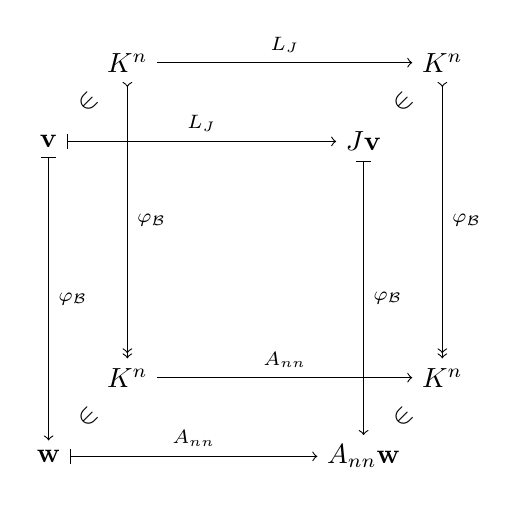
\begin{tikzpicture}[auto]

    \node (a) at (1, 1) {$K^n $};
    \node (b) at (5, 1) {$K^n $};
    \node (c) at (1, 5) {$K^n $};
    \node (d) at (5, 5) {$K^n $};
    \node (e) at (0, 4) {${\bf v} $};
    \node (f) at (4, 4) {$J {\bf v} $};
    \node (g) at (0.5, 4.5) {\rotatebox{45}{$\scriptsize \in $} };
    \node (h) at (4.5, 4.5) {\rotatebox{45}{$\scriptsize \in $} };
    \node (i) at (0, 0) {${\bf w} $};
    \node (j) at (4, 0) {$A_{nn} {\bf w} $};
    \node (k) at (0.5, 0.5) {\rotatebox{45}{$\in $} };
    \node (l) at (4.5, 0.5) {\rotatebox{45}{$\in $} };
    
    \draw [->] (c) to node {$\scriptstyle L_J $} (d);
    \draw [|->] (e) to node {$\scriptstyle L_J $} (f);
    \draw [>->>] (c) to node {$\scriptstyle \varphi_{{\mathcal B} } $} (a);
    \draw [|->] (e) to node {$\scriptstyle \varphi_{{\mathcal B} } $} (i);
    \draw [->] (a) to node {$\scriptstyle A_{nn} $} (b);
    \draw [|->] (i) to node {$\scriptstyle A_{nn} $} (j);
    \draw [>->>] (d) to node {$\scriptstyle \varphi_{{\mathcal B} } $} (b);
    \draw [|->] (f) to node {$\scriptstyle \varphi_{{\mathcal B} } $} (j);
    
  \end{tikzpicture} 
\end{center}
その基底$\mathcal{B}$に関する基底変換における線形同型写像$\varphi_{\mathcal{B}}$がまさしくその行列$P$が対応する行列であるような線形写像である。ここで、正規直交基底を$\varepsilon$とおけば次のようになる。
\begin{align*}
J &= \left[ L_{A_{nn}} \right]_{\mathcal{B}}^{\mathcal{B}}\\
&= \left[ \varphi_{\mathcal{B}}^{- 1} \circ L_{J} \circ \varphi_{\mathcal{B}} \right]_{\mathcal{B}}^{\mathcal{B}}\\
&= \left[ \varphi_{\mathcal{B}}^{- 1} \right]_{\mathcal{B}}^{\varepsilon}\left[ L_{A_{nn}} \right]_{\varepsilon}^{\varepsilon}\left[ \varphi_{\mathcal{B}} \right]_{\varepsilon}^{\mathcal{B}}\\
&= {\left[ \varphi_{\mathcal{B}} \right]_{\varepsilon}^{\mathcal{B}}}^{- 1}\left[ L_{A_{nn}} \right]_{\varepsilon}^{\varepsilon}\left[ \varphi_{\mathcal{B}} \right]_{\varepsilon}^{\mathcal{B}}\\
&= P^{- 1}A_{nn}P
\end{align*}\par
ここで、そのJordan標準形$J$は次式のように表されることができるので、
\begin{align*}
J = \begin{pmatrix}
J\left( \lambda_{1};q_{1} \right) & \  & \  & O \\
\  & J\left( \lambda_{2};q_{2} \right) & \  & \  \\
\  & \  & \ddots & \  \\
O & \  & \  & J\left( \lambda_{s};q_{s} \right) \\
\end{pmatrix}
\end{align*}
次のようになる、
\begin{align*}
\begin{pmatrix}
A_{nn}P_{1} & A_{nn}P_{2} & \cdots & A_{nn}P_{s} \\
\end{pmatrix} &= A_{nn}\begin{pmatrix}
P_{1} & P_{2} & \cdots & P_{s} \\
\end{pmatrix}\\
&= A_{nn}P\\
&= PP^{- 1}A_{nn}P\\
&= PJ\\
&= \begin{pmatrix}
P_{1} & P_{2} & \cdots & P_{s} \\
\end{pmatrix}\begin{pmatrix}
J\left( \lambda_{1};q_{1} \right) & \  & \  & O \\
\  & J\left( \lambda_{2};q_{2} \right) & \  & \  \\
\  & \  & \ddots & \  \\
O & \  & \  & J\left( \lambda_{s};q_{s} \right) \\
\end{pmatrix}\\
&= \begin{pmatrix}
P_{1}J\left( \lambda_{1};q_{1} \right) & P_{2}J\left( \lambda_{2};q_{2} \right) & \cdots & P_{s}J\left( \lambda_{s};q_{s} \right) \\
\end{pmatrix}
\end{align*}
即ち、$\forall i \in \varLambda_{s}$に対し、$A_{nn}P_{i} = P_{i}J\left( \lambda_{i};q_{i} \right)$が成り立つ。これが成り立つならそのときに限り、次のようになる、
\begin{align*}
\begin{pmatrix}
A_{nn}Q_{1} & A_{nn}Q_{2} & \cdots & A_{nn}Q_{r_{i}} \\
\end{pmatrix} &= A_{nn}\begin{pmatrix}
Q_{1} & Q_{2} & \cdots & Q_{r_{i}} \\
\end{pmatrix}\\
&= A_{nn}P_{i}\\
&= P_{i}J\left( \lambda_{i};q_{i} \right)\\
&= \begin{pmatrix}
Q_{1} & Q_{2} & \cdots & Q_{r_{i}} \\
\end{pmatrix} \cdot \begin{pmatrix}
J\left( \lambda_{i},q_{i1} \right) & \  & \  & O \\
\  & J\left( \lambda_{i},q_{i2} \right) & \  & \  \\
\  & \  & \ddots & \  \\
O & \  & \  & J\left( \lambda_{i},q_{ir_{i}} \right) \\
\end{pmatrix}\\
&= \begin{pmatrix}
Q_{1}J\left( \lambda_{i},q_{i1} \right) & Q_{2}J\left( \lambda_{i},q_{i2} \right) & \cdots & Q_{r_{i}}J\left( \lambda_{i},q_{ir_{i}} \right) \\
\end{pmatrix}
\end{align*}
即ち、$\forall i \in \varLambda_{s}\forall j \in \varLambda_{r_{i}}$に対し、$A_{nn}Q_{j} = Q_{j}J\left( \lambda_{i},q_{ij} \right)$が成り立つ。これが成り立つならそのときに限り、次のようになる、
\begin{align*}
\begin{pmatrix}
A_{nn}\mathbf{p}_{ij1} & A_{nn}\mathbf{p}_{ij2} & \cdots & A_{nn}\mathbf{p}_{ijq_{ij}} \\
\end{pmatrix} &= A_{nn}\begin{pmatrix}
\mathbf{p}_{ij1} & \mathbf{p}_{ij2} & \cdots & \mathbf{p}_{ijq_{ij}} \\
\end{pmatrix}\\
&= A_{nn}Q_{j}\\
&= Q_{j}J\left( \lambda_{i},q_{ij} \right)\\
&= \begin{pmatrix}
\mathbf{p}_{ij1} & \mathbf{p}_{ij2} & \cdots & \mathbf{p}_{ijq_{ij}} \\
\end{pmatrix}\begin{pmatrix}
\lambda_{i} & 1 & \  & \  & O \\
\  & \lambda_{i} & 1 & \  & \  \\
\  & \  & \lambda_{i} & \ddots & \  \\
\  & \  & \  & \ddots & 1 \\
O & \  & \  & \  & \lambda_{i} \\
\end{pmatrix}\\
&= \begin{pmatrix}
\lambda_{i}\mathbf{p}_{ij1} & \mathbf{p}_{ij1} + \lambda_{i}\mathbf{p}_{ij2} & \cdots & \mathbf{p}_{ij,q_{ij} - 1} + \lambda_{i}\mathbf{p}_{ijq_{ij}} \\
\end{pmatrix}
\end{align*}
即ち、次式が得られる。
\begin{align*}
\left\{ \begin{matrix}
\left( A_{nn} - \lambda_{i}I_{n} \right)\mathbf{p}_{ij1} = \mathbf{0} \\
\left( A_{nn} - \lambda_{i}I_{n} \right)\mathbf{p}_{ij2} = \mathbf{p}_{ij1} \\
 \vdots \\
\left( A_{nn} - \lambda_{i}I_{n} \right)\mathbf{p}_{ijq_{ij}} = \mathbf{p}_{ij,q_{ij} - 1} \\
\end{matrix} \right.\ 
\end{align*}
\end{proof}\par
この定理により、その変換行列$P$を求めるのに、上の連立1次方程式を求めることに帰着できる。そこで、$\forall i \in \varLambda_{s}\forall j \in \varLambda_{r_{i}}\forall k \in \varLambda_{q_{ij} - 1}$に対し、$\mathbf{p}_{ijk} \neq \mathbf{0}$が成り立つことから、次のような2通りの求め方がある。
\begin{itemize}
\item
  1つ目は、$\forall i \in \varLambda_{s}\forall j \in \varLambda_{r_{i}}$に対し、$\left( A_{nn} - \lambda_{i}I_{n} \right)^{q_{ij}}\mathbf{v}_{ij} = \mathbf{0}$かつ$\left( A_{nn} - \lambda_{i}I_{n} \right)^{q_{ij} - 1}\mathbf{v}_{ij} \neq \mathbf{0}$なるvector$\mathbf{v}_{ij}$をまず求め、次のように順次vectors$\mathbf{p}_{ijk}$を求めていく方法である。
\begin{align*}
\mathbf{v}_{ij} &= \mathbf{p}_{ijq_{ij}}\\
\left( A_{nn} - \lambda_{i}I_{n} \right)\mathbf{p}_{ijq_{ij}} &= \mathbf{p}_{ij,q_{ij} - 1}\\
&\vdots \\
\left( A_{nn} - \lambda_{i}I_{n} \right)\mathbf{p}_{ij2} &= \mathbf{p}_{ij1}
\end{align*}
なお、ここで、$i \in \varLambda_{s}$、$j \in \varLambda_{r_{i}}$なるvectors$\mathbf{v}_{ij}$が線形独立となるようにとることに注意されたい。
\item
  2つ目は、$\forall i \in \varLambda_{s}\forall j \in \varLambda_{r_{i}}$に対し、$\mathbf{p}_{ij0} = \mathbf{0}$として、$\forall k \in \varLambda_{q_{ij}} \setminus \left\{ 1 \right\}$に対し、vector$\mathbf{p}_{ij,k - 1}$が得られたとき、有解条件より連立1次方程式$\left( A_{nn} - \lambda_{i}I_{n} \right)\mathbf{x} = \mathbf{b}$が解をもつようなvector$\mathbf{b}$の条件$p(\mathbf{b})$を求めておき、連立1次方程式$\left( A_{nn} - \lambda_{i}I_{n} \right)\mathbf{x} = \mathbf{p}_{ij,k - 1}$なる非自明な解$\mathbf{x}$を含む解空間$K_{k}$を求めその解空間$K_{k}$の元$\mathbf{b}$のうちこの条件$p\left( \mathbf{b} \right)$を満たすようなvector$\mathbf{x}$を選びこれを$\mathbf{x} = \mathbf{p}_{ijk}$とおく方法である。ただし、vector$\mathbf{p}_{ijq_{ij}}$はこの条件$p\left( \mathbf{b} \right)$を満たす必要はないことに注意されたい。さらに、$i \in \varLambda_{s}$、$j \in \varLambda_{r_{i}}$なるvectors$\mathbf{p}_{ij1}$が線形独立となるようにとることに注意されたい。
\end{itemize}\par
例えば、次の行列$A$のJordan標準形$J$とその変換行列$P$を求めよう。
\begin{align*}
A = \begin{pmatrix}
0 & - 1 & - 1 & 1 \\
 - 1 & - 2 & - 2 & 2 \\
 - 1 & - 1 & 0 & 1 \\
 - 3 & - 7 & - 5 & 6 \\
\end{pmatrix}
\end{align*}
この特性$X$-行列$XI - A$の単因子標準形を求めよう。したがって、次のようになる。
\begin{align*}
XI - A &= \begin{pmatrix}
X & 1 & 1 & - 1 \\
1 & X + 2 & 2 & - 2 \\
1 & 1 & X & - 1 \\
3 & 7 & 5 & X - 6 \\
\end{pmatrix} \rightarrow \begin{pmatrix}
1 & 1 & X & - 1 \\
 - 1 & - X - 2 & - 2 & 2 \\
 - 3 & - 7 & - 5 & - X + 6 \\
 - X & - 1 & - 1 & 1 \\
\end{pmatrix}\\
&\rightarrow \begin{pmatrix}
1 & 1 & X & - 1 \\
0 & - X - 1 & X - 2 & 1 \\
0 & - 4 & 3X - 5 & - X + 3 \\
0 & X - 1 & X^{2} - 1 & X + 1 \\
\end{pmatrix}\\
&\rightarrow \begin{pmatrix}
1 & 0 & 0 & 0 \\
0 & 4 & - 3X + 5 & X - 3 \\
0 & - 4X - 4 & 4X - 8 & 4 \\
0 & - 4X + 4 & - 4X^{2} + 4 & - 4X - 4 \\
\end{pmatrix}\\
&\rightarrow \begin{pmatrix}
1 & 0 & 0 & 0 \\
0 & 1 & 0 & 0 \\
0 & 0 & - 3X^{2} + 6X - 3 & X^{2} - 2X + 1 \\
0 & 0 & - 7X^{2} + 8X - 1 & X^{2} - 1 \\
\end{pmatrix}\\
&\rightarrow \begin{pmatrix}
1 & 0 & 0 & 0 \\
0 & 1 & 0 & 0 \\
0 & 0 & X - 1 & - 2X^{2} + X + 1 \\
0 & 0 & X^{2} - 1 & - 7X^{2} + 8X - 1 \\
\end{pmatrix}\\
&\rightarrow \begin{pmatrix}
1 & 0 & 0 & 0 \\
0 & 1 & 0 & 0 \\
0 & 0 & X - 1 & - 2X^{2} + X + 1 \\
0 & 0 & 0 & 2X^{3} - 6X^{2} + 6X - 2 \\
\end{pmatrix}\\
&\rightarrow \begin{pmatrix}
1 & 0 & 0 & 0 \\
0 & 1 & 0 & 0 \\
0 & 0 & X - 1 & - (2X + 1)(X - 1) \\
0 & 0 & 0 & (X - 1)^{3} \\
\end{pmatrix}\\
&\rightarrow \begin{pmatrix}
1 & 0 & 0 & 0 \\
0 & 1 & 0 & 0 \\
0 & 0 & X - 1 & 0 \\
0 & 0 & 0 & (X - 1)^{3} \\
\end{pmatrix}
\end{align*}
したがって、求めるJordan標準形$J$は次のように与えられる。
\begin{align*}
J = \begin{pmatrix}
1 & 0 & 0 & 0 \\
0 & 1 & 1 & 0 \\
0 & 0 & 1 & 1 \\
0 & 0 & 0 & 1 \\
\end{pmatrix}
\end{align*}\par
ここで、$J = P^{- 1}AP$が成り立つことから、$P = \begin{pmatrix}
\mathbf{p}_{1} & \mathbf{p}_{2} & \mathbf{p}_{3} & \mathbf{p}_{4} \\
\end{pmatrix}$とおかれれば、次のようになる。
\begin{align*}
J = P^{- 1}AP &\Leftrightarrow AP = PJ\\
&\Leftrightarrow A\begin{pmatrix}
\mathbf{p}_{1} & \mathbf{p}_{2} & \mathbf{p}_{3} & \mathbf{p}_{4} \\
\end{pmatrix} = \begin{pmatrix}
\mathbf{p}_{1} & \mathbf{p}_{2} & \mathbf{p}_{3} & \mathbf{p}_{4} \\
\end{pmatrix}J\\
&\Leftrightarrow \begin{pmatrix}
A\mathbf{p}_{1} & A\mathbf{p}_{2} & A\mathbf{p}_{3} & A\mathbf{p}_{4} \\
\end{pmatrix} = \begin{pmatrix}
\mathbf{p}_{1} & \mathbf{p}_{2} & \mathbf{p}_{3} & \mathbf{p}_{4} \\
\end{pmatrix}\begin{pmatrix}
1 & 0 & 0 & 0 \\
0 & 1 & 1 & 0 \\
0 & 0 & 1 & 1 \\
0 & 0 & 0 & 1 \\
\end{pmatrix}\\
&\Leftrightarrow \begin{pmatrix}
A\mathbf{p}_{1} & A\mathbf{p}_{2} & A\mathbf{p}_{3} & A\mathbf{p}_{4} \\
\end{pmatrix} = \begin{pmatrix}
\mathbf{p}_{1} & \mathbf{p}_{2} & \mathbf{p}_{2} + \mathbf{p}_{3} & \mathbf{p}_{3} + \mathbf{p}_{4} \\
\end{pmatrix}\\
&\Leftrightarrow \left\{ \begin{matrix}
(A - I)\mathbf{p}_{1} = \mathbf{0} \\
(A - I)\mathbf{p}_{2} = \mathbf{0} \\
(A - I)\mathbf{p}_{3} = \mathbf{p}_{2} \\
(A - I)\mathbf{p}_{4} = \mathbf{p}_{3} \\
\end{matrix} \right.
\end{align*}
ここで、$(A - I)^{3} = O$はもちろん成り立つことに注意すると、次のようになることから、
\begin{align*}
(A - I)^{2} = \begin{pmatrix}
 - 1 & - 1 & - 1 & 1 \\
 - 1 & - 3 & - 2 & 2 \\
 - 1 & - 1 & - 1 & 1 \\
 - 3 & - 7 & - 5 & 5 \\
\end{pmatrix}^{2} = \begin{pmatrix}
0 & - 2 & - 1 & 1 \\
0 & - 2 & - 1 & 1 \\
0 & - 2 & - 1 & 1 \\
0 & - 6 & - 3 & 3 \\
\end{pmatrix}
\end{align*}
$(A - I)^{3}\mathbf{v} = \mathbf{0}$かつ$(A - I)^{2}\mathbf{v} \neq \mathbf{0}$なるvector$\mathbf{v}$として、次式のようにおくと、
\begin{align*}
\mathbf{p}_{4} = \begin{pmatrix}
0 \\
1 \\
0 \\
0 \\
\end{pmatrix}
\end{align*}
次のようになる。
\begin{align*}
\mathbf{p}_{3} &= (A - I)\mathbf{p}_{4} = \begin{pmatrix}
 - 1 & - 1 & - 1 & 1 \\
 - 1 & - 3 & - 2 & 2 \\
 - 1 & - 1 & - 1 & 1 \\
 - 3 & - 7 & - 5 & 5 \\
\end{pmatrix}\begin{pmatrix}
0 \\
1 \\
0 \\
0 \\
\end{pmatrix} = \begin{pmatrix}
 - 1 \\
 - 3 \\
 - 1 \\
 - 7 \\
\end{pmatrix}\\
\mathbf{p}_{2} &= (A - I)\mathbf{p}_{3} = \begin{pmatrix}
 - 1 & - 1 & - 1 & 1 \\
 - 1 & - 3 & - 2 & 2 \\
 - 1 & - 1 & - 1 & 1 \\
 - 3 & - 7 & - 5 & 5 \\
\end{pmatrix}\begin{pmatrix}
 - 1 \\
 - 3 \\
 - 1 \\
 - 7 \\
\end{pmatrix} = \begin{pmatrix}
 - 2 \\
 - 2 \\
 - 2 \\
 - 6 \\
\end{pmatrix}
\end{align*}\par
次に、$(A - I)\mathbf{v} = \mathbf{0}$かつ$(A - I)^{0}\mathbf{v} = \mathbf{v} \neq \mathbf{0}$なるなるvector$\mathbf{v}$として、次式のようにおくと、
\begin{align*}
\mathbf{p}_{1} = \begin{pmatrix}
 - 1 \\
 - 1 \\
2 \\
0 \\
\end{pmatrix}
\end{align*}
これらのvectors$\mathbf{p}_{1}$、$\mathbf{p}_{2}$、$\mathbf{p}_{3}$、$\mathbf{p}_{4}$は線形独立である。したがって、求める行列$P$は次のように与えられる。
\begin{align*}
P = \begin{pmatrix}
 - 1 & - 2 & - 1 & 0 \\
 - 1 & - 2 & - 3 & 1 \\
2 & - 2 & - 1 & 0 \\
0 & - 6 & - 7 & 0 \\
\end{pmatrix}
\end{align*}
したがって、次のようになる。
\begin{align*}
\begin{pmatrix}
1 & 0 & 0 & 0 \\
0 & 1 & 1 & 0 \\
0 & 0 & 1 & 1 \\
0 & 0 & 0 & 1 \\
\end{pmatrix} = \begin{pmatrix}
 - 1 & - 2 & - 1 & 0 \\
 - 1 & - 2 & - 3 & 1 \\
2 & - 2 & - 1 & 0 \\
0 & - 6 & - 7 & 0 \\
\end{pmatrix}^{- 1}\begin{pmatrix}
0 & - 1 & - 1 & 1 \\
 - 1 & - 2 & - 2 & 2 \\
 - 1 & - 1 & 0 & 1 \\
 - 3 & - 7 & - 5 & 6 \\
\end{pmatrix}\begin{pmatrix}
 - 1 & - 2 & - 1 & 0 \\
 - 1 & - 2 & - 3 & 1 \\
2 & - 2 & - 1 & 0 \\
0 & - 6 & - 7 & 0 \\
\end{pmatrix}
\end{align*}\par
別の方法でその行列$P$を求めよう。まずは、連立1次方程式$(A - I)\mathbf{x} = \mathbf{b}$が解をもつようなvector$\mathbf{b}$の条件$p(\mathbf{b})$を求めよう。次のようにおかれれば、
\begin{align*}
\mathbf{b} = \begin{pmatrix}
x \\
y \\
z \\
w \\
\end{pmatrix}
\end{align*}
$(A - I)\mathbf{x} = \mathbf{b}$と$\begin{pmatrix}
A - I & \mathbf{b} \\
\end{pmatrix}\begin{pmatrix}
\mathbf{x} \\
 - 1 \\
\end{pmatrix} = \mathbf{0}$とは同値である。したがって、次のようになることから、
\begin{align*}
\begin{pmatrix}
A - I & \mathbf{b} \\
\end{pmatrix} &= \begin{pmatrix}
 - 1 & - 1 & - 1 & 1 & x \\
 - 1 & - 3 & - 2 & 2 & y \\
 - 1 & - 1 & - 1 & 1 & z \\
 - 3 & - 7 & - 5 & 5 & w \\
\end{pmatrix} \rightarrow \begin{pmatrix}
 - 1 & - 1 & - 1 & 1 & x \\
0 & - 2 & - 1 & 1 & y - x \\
0 & 0 & 0 & 0 & z - x \\
0 & - 4 & - 2 & 2 & w - 3x \\
\end{pmatrix}\\
&\rightarrow \begin{pmatrix}
 - 1 & - 1 & - 1 & 1 & x \\
0 & 2 & 1 & - 1 & x - y \\
0 & 0 & 0 & 0 & z - x \\
0 & 0 & 0 & 0 & (w - 3x) + 2(x - y) \\
\end{pmatrix}\\
&\rightarrow \begin{pmatrix}
2 & 2 & 2 & - 2 & - 2x \\
0 & 2 & 1 & - 1 & x - y \\
0 & 0 & 0 & 0 & - x + z \\
0 & 0 & 0 & 0 & - x - 2y + w \\
\end{pmatrix}\\
&\rightarrow \begin{pmatrix}
2 & 0 & 1 & - 1 & - 3x + y \\
0 & 2 & 1 & - 1 & x - y \\
0 & 0 & 0 & 0 & - x + z \\
0 & 0 & 0 & 0 & - x - 2y + w \\
\end{pmatrix}\\
&\rightarrow \begin{pmatrix}
1 & 0 & \frac{1}{2} & - \frac{1}{2} & - \frac{3x}{2} + \frac{y}{2} \\
0 & 1 & \frac{1}{2} & - \frac{1}{2} & \frac{x}{2} - \frac{y}{2} \\
0 & 0 & 0 & 0 & - x + z \\
0 & 0 & 0 & 0 & - x - 2y + w \\
\end{pmatrix}
\end{align*}
有解条件より${\mathrm{rank}}(A - I) = {\mathrm{rank}}\begin{pmatrix}
A - I & \mathbf{b} \\
\end{pmatrix}$が成り立つならそのときに限り、その連立1次方程式$(A - I)\mathbf{x} = \mathbf{b}$が解をもつので、$- x + z = 0$かつ$- x - 2y + w = 0$が成り立つ。\par
次に、連立$1$次方程式$(A - I)\mathbf{x} = \mathbf{0}$の解空間$K_{2}$を求めよう。上記と同様にして次のようになることから、
\begin{align*}
A - I = \begin{pmatrix}
 - 1 & - 1 & - 1 & 1 \\
 - 1 & - 3 & - 2 & 2 \\
 - 1 & - 1 & - 1 & 1 \\
 - 3 & - 7 & - 5 & 5 \\
\end{pmatrix} \rightarrow \begin{pmatrix}
1 & 0 & \frac{1}{2} & - \frac{1}{2} \\
0 & 1 & \frac{1}{2} & - \frac{1}{2} \\
0 & 0 & 0 & 0 \\
0 & 0 & 0 & 0 \\
\end{pmatrix}
\end{align*}
次式が成り立つ。
\begin{align*}
K_{2} = {\mathrm{span}}\left\{ \begin{pmatrix}
 - 1 \\
 - 1 \\
2 \\
0 \\
\end{pmatrix},\begin{pmatrix}
1 \\
1 \\
0 \\
2 \\
\end{pmatrix} \right\},\ \ \mathbf{x} = \begin{pmatrix}
 - s + t \\
 - s + t \\
2s \\
2t \\
\end{pmatrix}
\end{align*}
これのうち、その連立1次方程式$(A - I)\mathbf{x}' = \mathbf{x}$が解をもつならそのときに限り、上記の議論により$- ( - s + t) + 2s = 0$かつ$- ( - s + t) - 2( - s + t) + 2t = 0$が成り立つことになる。これにより、$3s = t$が成り立つようなvector$\mathbf{x}$として次のようにおく。
\begin{align*}
\mathbf{x} = \begin{pmatrix}
2 \\
2 \\
2 \\
6 \\
\end{pmatrix} = \mathbf{p}_{2}
\end{align*}\par
このときの連立$1$次方程式$(A - I)\mathbf{x} = \mathbf{p}_{2}$の解空間$K_{3}$を求めよう。上記と同様にして次のようになることから、
\begin{align*}
\begin{pmatrix}
A - I & \mathbf{b} \\
\end{pmatrix} = \begin{pmatrix}
 - 1 & - 1 & - 1 & 1 & 2 \\
 - 1 & - 3 & - 2 & 2 & 2 \\
 - 1 & - 1 & - 1 & 1 & 2 \\
 - 3 & - 7 & - 5 & 5 & 6 \\
\end{pmatrix} \rightarrow \begin{pmatrix}
1 & 0 & \frac{1}{2} & - \frac{1}{2} & - 2 \\
0 & 1 & \frac{1}{2} & - \frac{1}{2} & 0 \\
0 & 0 & 0 & 0 & 0 \\
0 & 0 & 0 & 0 & 0 \\
\end{pmatrix}
\end{align*}
次式が成り立つ。
\begin{align*}
K_{3} = {\mathrm{span}}\left\{ \begin{pmatrix}
 - 1 \\
 - 1 \\
2 \\
0 \\
\end{pmatrix},\begin{pmatrix}
1 \\
1 \\
0 \\
2 \\
\end{pmatrix} \right\} + \begin{pmatrix}
 - 2 \\
0 \\
0 \\
0 \\
\end{pmatrix},\ \ \mathbf{x} = \begin{pmatrix}
 - s + t - 2 \\
 - s + t \\
2s \\
2t \\
\end{pmatrix}
\end{align*}
これのうち、その連立1次方程式$(A - I)\mathbf{x}' = \mathbf{x}$が解をもつならそのときに限り、上記の議論により$- ( - s + t - 2) + 2s = 0$かつ$- ( - s + t - 2) - 2( - s + t) + 2t = 0$が成り立つことになる。これにより、$3s + 2 = t$が成り立つようなvector$\mathbf{x}$として次のようにおく。
\begin{align*}
\mathbf{x} = \begin{pmatrix}
2 \\
4 \\
2 \\
10 \\
\end{pmatrix} = \mathbf{p}_{3}
\end{align*}\par
このときの連立$1$次方程式$(A - I)\mathbf{x} = \mathbf{p}_{3}$の解空間$K_{4}$を求めよう。上記と同様にして次のようになることから、
\begin{align*}
\begin{pmatrix}
A - I & \mathbf{b} \\
\end{pmatrix} = \begin{pmatrix}
 - 1 & - 1 & - 1 & 1 & 2 \\
 - 1 & - 3 & - 2 & 2 & 4 \\
 - 1 & - 1 & - 1 & 1 & 2 \\
 - 3 & - 7 & - 5 & 5 & 10 \\
\end{pmatrix} \rightarrow \begin{pmatrix}
1 & 0 & \frac{1}{2} & - \frac{1}{2} & - 2 \\
0 & 1 & \frac{1}{2} & - \frac{1}{2} & 0 \\
0 & 0 & 0 & 0 & 0 \\
0 & 0 & 0 & 0 & 0 \\
\end{pmatrix}
\end{align*}
次式が成り立つ。
\begin{align*}
K_{3} = {\mathrm{span}}\left\{ \begin{pmatrix}
 - 1 \\
 - 1 \\
2 \\
0 \\
\end{pmatrix},\begin{pmatrix}
1 \\
1 \\
0 \\
2 \\
\end{pmatrix} \right\} + \begin{pmatrix}
 - 1 \\
 - 1 \\
0 \\
0 \\
\end{pmatrix},\ \ \mathbf{x} = \begin{pmatrix}
 - s + t - 1 \\
 - s + t - 1 \\
2s \\
2t \\
\end{pmatrix}
\end{align*}
これにより、次のようにおく。
\begin{align*}
\mathbf{p}_{4} = \begin{pmatrix}
 - 1 \\
 - 1 \\
2 \\
2 \\
\end{pmatrix}
\end{align*}\par
最後に、$(A - I)\mathbf{x} = \mathbf{0}$の解空間$K_{1}$を求めよう。これはすでに次のように与えられている。
\begin{align*}
K_{1} = {\mathrm{span}}\left\{ \begin{pmatrix}
 - 1 \\
 - 1 \\
2 \\
0 \\
\end{pmatrix},\begin{pmatrix}
1 \\
1 \\
0 \\
2 \\
\end{pmatrix} \right\},\ \ \mathbf{x} = \begin{pmatrix}
 - s + t \\
 - s + t \\
2s \\
2t \\
\end{pmatrix}
\end{align*}
これにより、次のようにおく。
\begin{align*}
\mathbf{p}_{1} = \begin{pmatrix}
0 \\
0 \\
2 \\
2 \\
\end{pmatrix}
\end{align*}
これらのvectors$\mathbf{p}_{1}$、$\mathbf{p}_{2}$、$\mathbf{p}_{3}$、$\mathbf{p}_{4}$は線形独立である。したがって、求める行列$P$は次のように与えられる。
\begin{align*}
P = \begin{pmatrix}
0 & 2 & 2 & - 1 \\
0 & 2 & 4 & - 1 \\
2 & 2 & 2 & 2 \\
2 & 6 & 10 & 2 \\
\end{pmatrix}
\end{align*}
したがって、次のようになる。
\begin{align*}
\begin{pmatrix}
1 & 0 & 0 & 0 \\
0 & 1 & 1 & 0 \\
0 & 0 & 1 & 1 \\
0 & 0 & 0 & 1 \\
\end{pmatrix} = \begin{pmatrix}
0 & 2 & 2 & - 1 \\
0 & 2 & 4 & - 1 \\
2 & 2 & 2 & 2 \\
2 & 6 & 10 & 2 \\
\end{pmatrix}^{- 1}\begin{pmatrix}
0 & - 1 & - 1 & 1 \\
 - 1 & - 2 & - 2 & 2 \\
 - 1 & - 1 & 0 & 1 \\
 - 3 & - 7 & - 5 & 6 \\
\end{pmatrix}\begin{pmatrix}
0 & 2 & 2 & - 1 \\
0 & 2 & 4 & - 1 \\
2 & 2 & 2 & 2 \\
2 & 6 & 10 & 2 \\
\end{pmatrix}
\end{align*}
\begin{thebibliography}{50}
\bibitem{1}
  対馬龍司, 線形代数学講義, 共立出版, 2007. 改訂版8刷 p208-229 ISBN978-4-320-11097-7
\bibitem{2}
  齋藤正彦, 線型代数入門, 東京大学出版会, 1966. 第21刷 p173-191 ISBN978-4-13-062001-7
\bibitem{3}
  桂田祐史. "線形代数ノート 桂田祐史". 明治大学. \url{http://nalab.mind.meiji.ac.jp/~mk/note/linear-algebra.pdf} (2021-10-8 14:00 取得)
\end{thebibliography}
\end{document}
